\chapter{ 
Measurement of the electron charge asymmetry with \unit{840}{\invpb} }

The measurement detailed in the previous chapter was performed with
\unit{36}{\invpb} of data from the full 2010 dataset. 
In this next chapter, the update to the measurement of the electron charge asymmetry in
inclusive \inclusiveWe production with \unit{840}{\invpb} is presented. 
The data was collected with the \ac{CMS} detector from collisions from the
first 2011 \ac{LHC} run (Run A) and corresponds to a 25 times increase in
statistics over the 2010 measurement.


The majority of the 2011 analysis is identical to the 2010 analysis,
however small changes to the metheodolgy have been implemented due to changes
in the luminosity and the increase in data in the 2011 \ac{LHC} run.

\section{Event Selection}
\subsection{Trigger}


\begin{table}[htbp]
  \begin{center}
    \leavevmode
     \begin{tabular}{ll} 
      Run Ranges & Trigger  \\
     \hline
     160404-161176 & HLT\_Ele27\_CaloIdVT\_CaloIsoT\_TrkIdT\_TrkIsoT\_v1  \\
     161217-163261 & HLT\_Ele32\_CaloIdVT\_CaloIsoT\_TrkIdT\_TrkIsoT\_v1  \\
     163270-163869 & HLT\_Ele32\_CaloIdVT\_CaloIsoT\_TrkIdT\_TrkIsoT\_v2  \\
     165088-165633 & HLT\_Ele32\_CaloIdVT\_CaloIsoT\_TrkIdT\_TrkIsoT\_v3  \\
     165970-166967 & HLT\_Ele32\_CaloIdVT\_CaloIsoT\_TrkIdT\_TrkIsoT\_v4  \\
     \end{tabular}

  \caption{Triggers used to select the data used in this measurement.}
  \label{asym840:triggers}

   \end{center}
\end{table}


The definitions of the triggers follows the same pattern as described in 
\SectionRef{asym36:triggerdef}.

Due to the increased luminosity in the 2011 Run A, the identifaction and
isolation cuts applied to the trigger have been tightened. The \PT cut applied
to the electon have been increased, first to \unit{27}{\GeV} and then in later
runs to \unit{32}{\GeV}.

\subsection{Electron Selection}


 \begin{table}[htbp]
   \begin{center}
     \leavevmode
     \begin{tabular}{lcc} 
       \multicolumn{1}{c}{Variable} & \multicolumn{1}{c}{cut value (barrel)}& \multicolumn{1}{c}{cut value (endcap)}\\
         \hline   
 \multicolumn{3}{l}{ID Cuts}\\ 
         H/E & 0.04 & 0.025 \\
         $\Delta\phi$ & 0.06 & 0.03 \\
         $\Delta\eta$ & 0.004 & 0.007  \\
         $\sigma_{\eta\eta}$ & 0.01 & 0.03 \\ \hline
 \multicolumn{3}{l}{Isolation Cuts}\\ 
   $ISO_{trk} / E_T $  & 0.09 & 0.04 \\
   $ISO_{ecal}/ E_T$  & 0.07 & 0.05 \\
   $ISO_{hcal}/ E_T$  & 0.10 & 0.025 \\ \hline
 \multicolumn{3}{l}{Conversion Rejection Cuts}\\ \hline
   Missing Hits  & \multicolumn{2}{c}{$\leq 0$}\\
   Dist $||$ Dcot   & \multicolumn{2}{c}{$>0.02$}\\
     \end{tabular}
     \caption{Electron selection variables and corresponding cut values.}
     \label{asym840:electronselection}
   \end{center}
 \end{table}

The electron transverse momentum cut is shifted up to \unit{35}{\GeV} due to
the trigger contraints. This is the only change with respect to the 2010
analysis on the electron selection, detailed in
\TableRef{asym840:electronselection}.

\subsection{Event Selection}
The event selection remains the same with respect to the 2010 measurement.
An Event is selected if if contains a single electron that passes all electron
selection.
To removed Drell-Yan events an event is vetoed if it contains a second lepton
(an electron passing a loose selecton, or an isolated muon) with $\PT > 
\unit{15}{\GeV}$

The Particle Flow \ETm distribution for the events that pass the event
selection, with $\PT > \unit{35}{\GeV}$ and $|\eta| < 2.4$ is shown in
\FigureRef{asym840:pfmet}.

\begin{figure}[htb]
  \centering
  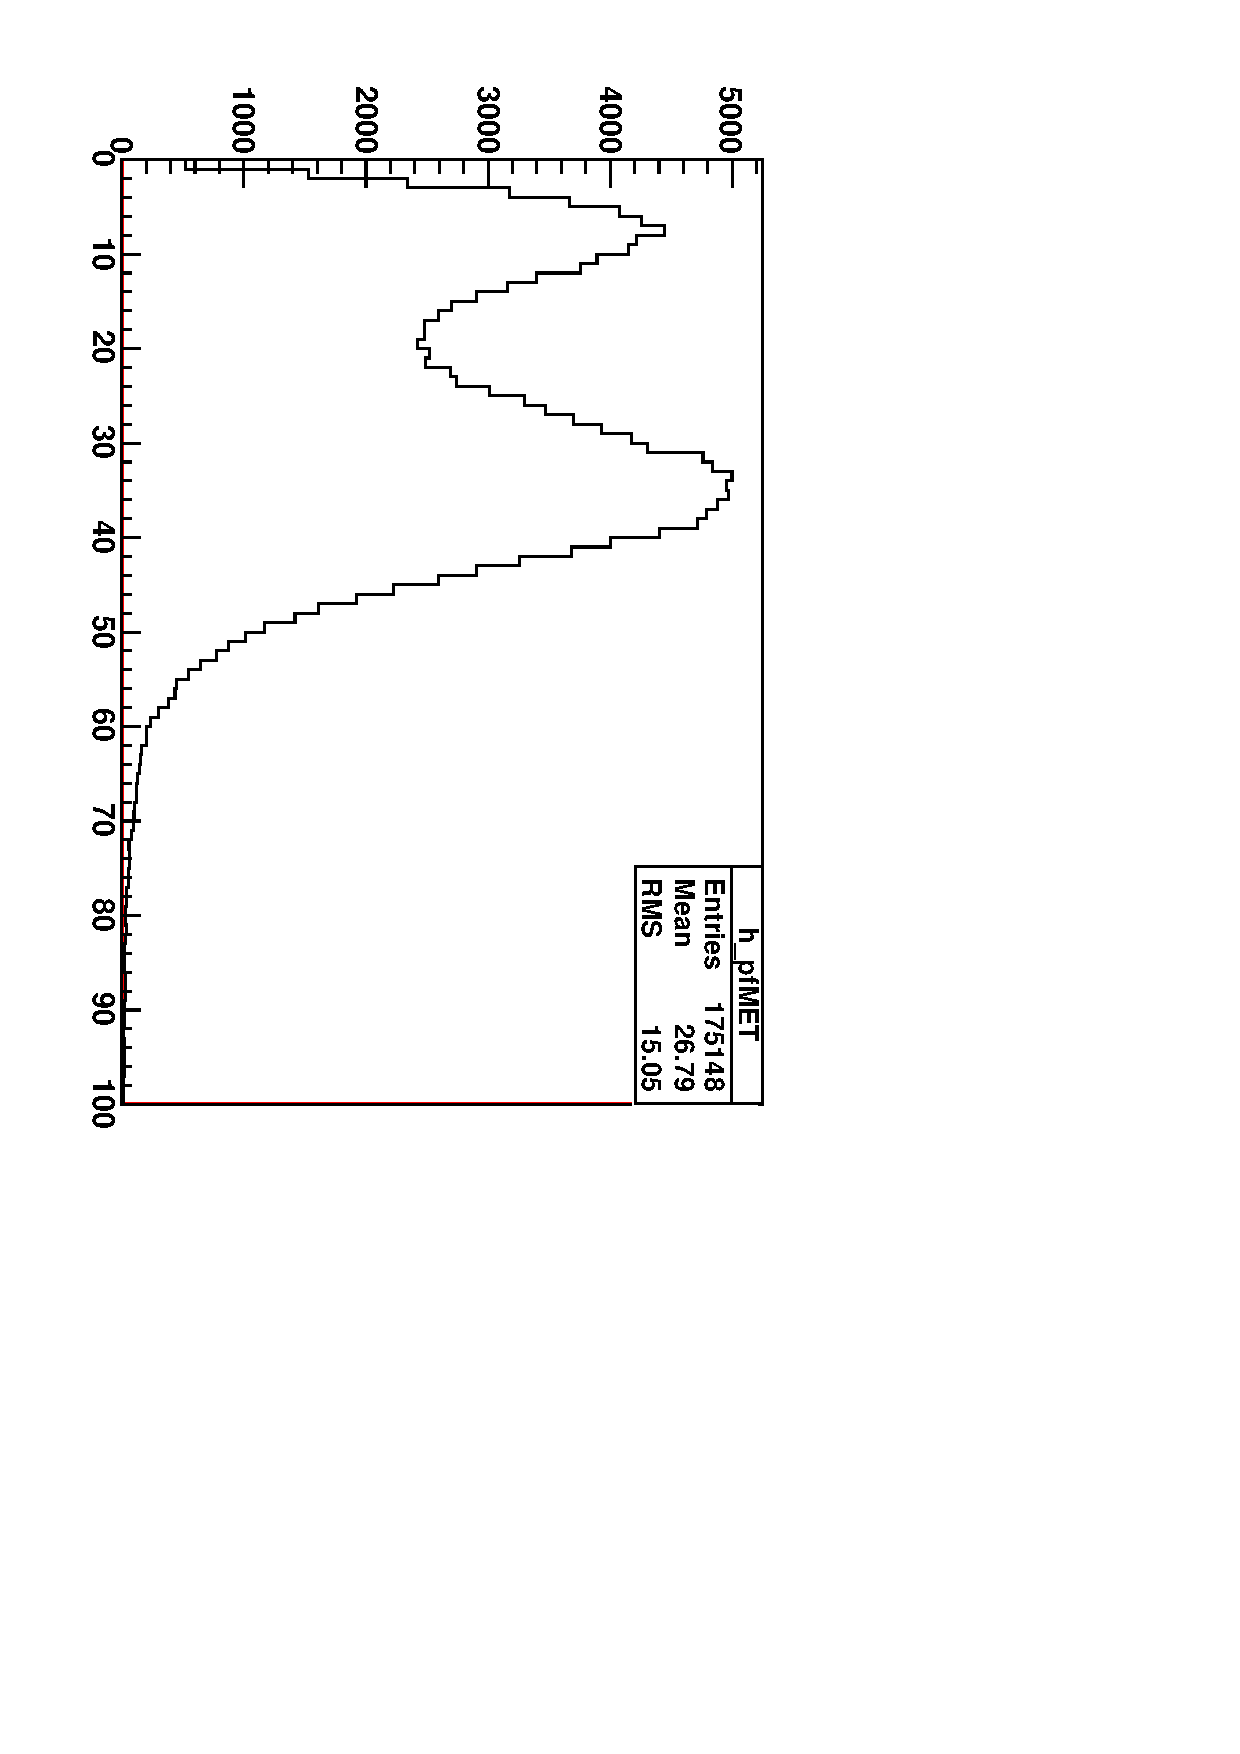
\includegraphics[width=0.5\textwidth]{pfmet}
  \caption{Particle Flow \ETm distribution for selected events.}
  \label{asym840:pfmet}
\end{figure}

The number of selected events that pass the event selection are shown in
\TableRef{asym36:selectedevents}.

\begin{table}[htb]
 \begin{center}
 \begin{tabular}{lcc}
 $|\eta|$ range & Selected Positrons & Selected Electrons\\
 \hline
 $0.0<| \eta |<0.2$ & 108235 &  90860 \\
 $0.2<| \eta |<0.4$ & 112870 &  93996 \\
 $0.4<| \eta |<0.6$ & 114148 &  94721 \\
 $0.6<| \eta |<0.8$ & 117099 &  95295 \\
 $0.8<| \eta |<1.0$ & 116956 &  94580 \\
 $1.0<| \eta |<1.2$ & 113336 &  90755 \\
 $1.2<| \eta |<1.4$ & 115265 &  91572 \\
 $1.6<| \eta |<1.8$ &  92137 &  70205 \\
 $1.8<| \eta |<2.0$ & 105596 &  80921 \\
 $2.0<| \eta |<2.2$ & 112419 &  86240 \\
 $2.2<| \eta |<2.4$ & 121224 & 102111 \\
 \end{tabular}
 \caption{Number of events passing the event selection for lepton momentum cut
 of \unit{\PT>35}{\GeV}.}
\label{asym840:selectedevents}
\end{center}
\end{table}

The exected composition of the selected events, derived from MC simulation
samples, is show in \TableRef{asym840:selectedcomp}. 

\begin{table}[htb]
\begin{center}
\begin{tabular}{lr}
& \unit{\PT>35}{\GeV}\\ \hline
$W\rightarrow e\nu$  & 76.2$\%$\\
QCD Background       & 16.0$\%$\\
EWK Total Background & 7.8$\%$ \\
~ EWK DYtautau      & 0.2$\%$  \\
~ EWK DYee          & 6.4$\%$  \\
~ EWK Wtaunu        & 0.8$\%$ \\
~ EWK ttbar         & 0.4$\%$ \\
\end{tabular}
\caption{Composition of selected events for lepton momentum cut of
  \unit{\PT>35}{\GeV}. Numbers are evaluated using simulation.}
 \label{asym840:selectedcomp}
\end{center}
\end{table}

\section{Signal Yield Extraction}
\todo[inline]{Summary of signal yield extraction method}

\subsection{QCD \ETm Shape}
\todo[inline]{background MET shape explanation. talk about antiselections in
some detail.}

\begin{table}[htbp]
  \begin{center}
    \leavevmode
    \begin{tabular}{lcc} 
      \multicolumn{1}{c}{Variable} & \multicolumn{1}{c}{cut value (barrel)}& \multicolumn{1}{c}{cut value (endcap)}\\\hline
        H/E & 0.04 & 0.025 \\
        $\Delta\phi$ & $>0.06$  & $>0.04$ \\
        $\Delta\eta$ & $>0.007$ & $>0.009$\\
  $ISO_{trk} / E_T $ & 0.09 & 0.04 \\
  $ISO_{ecal}/ E_T$  & 0.07 & 0.05 \\
  $ISO_{hcal}/ E_T$  & 0.10 & 0.025\\
    \end{tabular}
    \caption{Electron anti-selection variables and corresponding cut values. $\Delta\phi$ and $\Delta\eta$ cuts are inverted.}
    \label{asym840:AScuts}
  \end{center}
\end{table}

\subsection{Signal \ETm Shape from Boson Recoil}
\todo[inline]{Signal MET shape explanation. Quite a bit can be written here
about the boson recoil.}

\subsection{EWK \ETm Shape}
\todo[inline]{EWK MET shape explanation}


\subsection{Validation of Signal Extraction Method on Simulation}
\todo[inline]{pseudo data trials}

\subsection{Fit on Real Data}
\todo[inline]{Fit applied to data and uncorrected results.}

\begin{figure}
  \begin{center}
    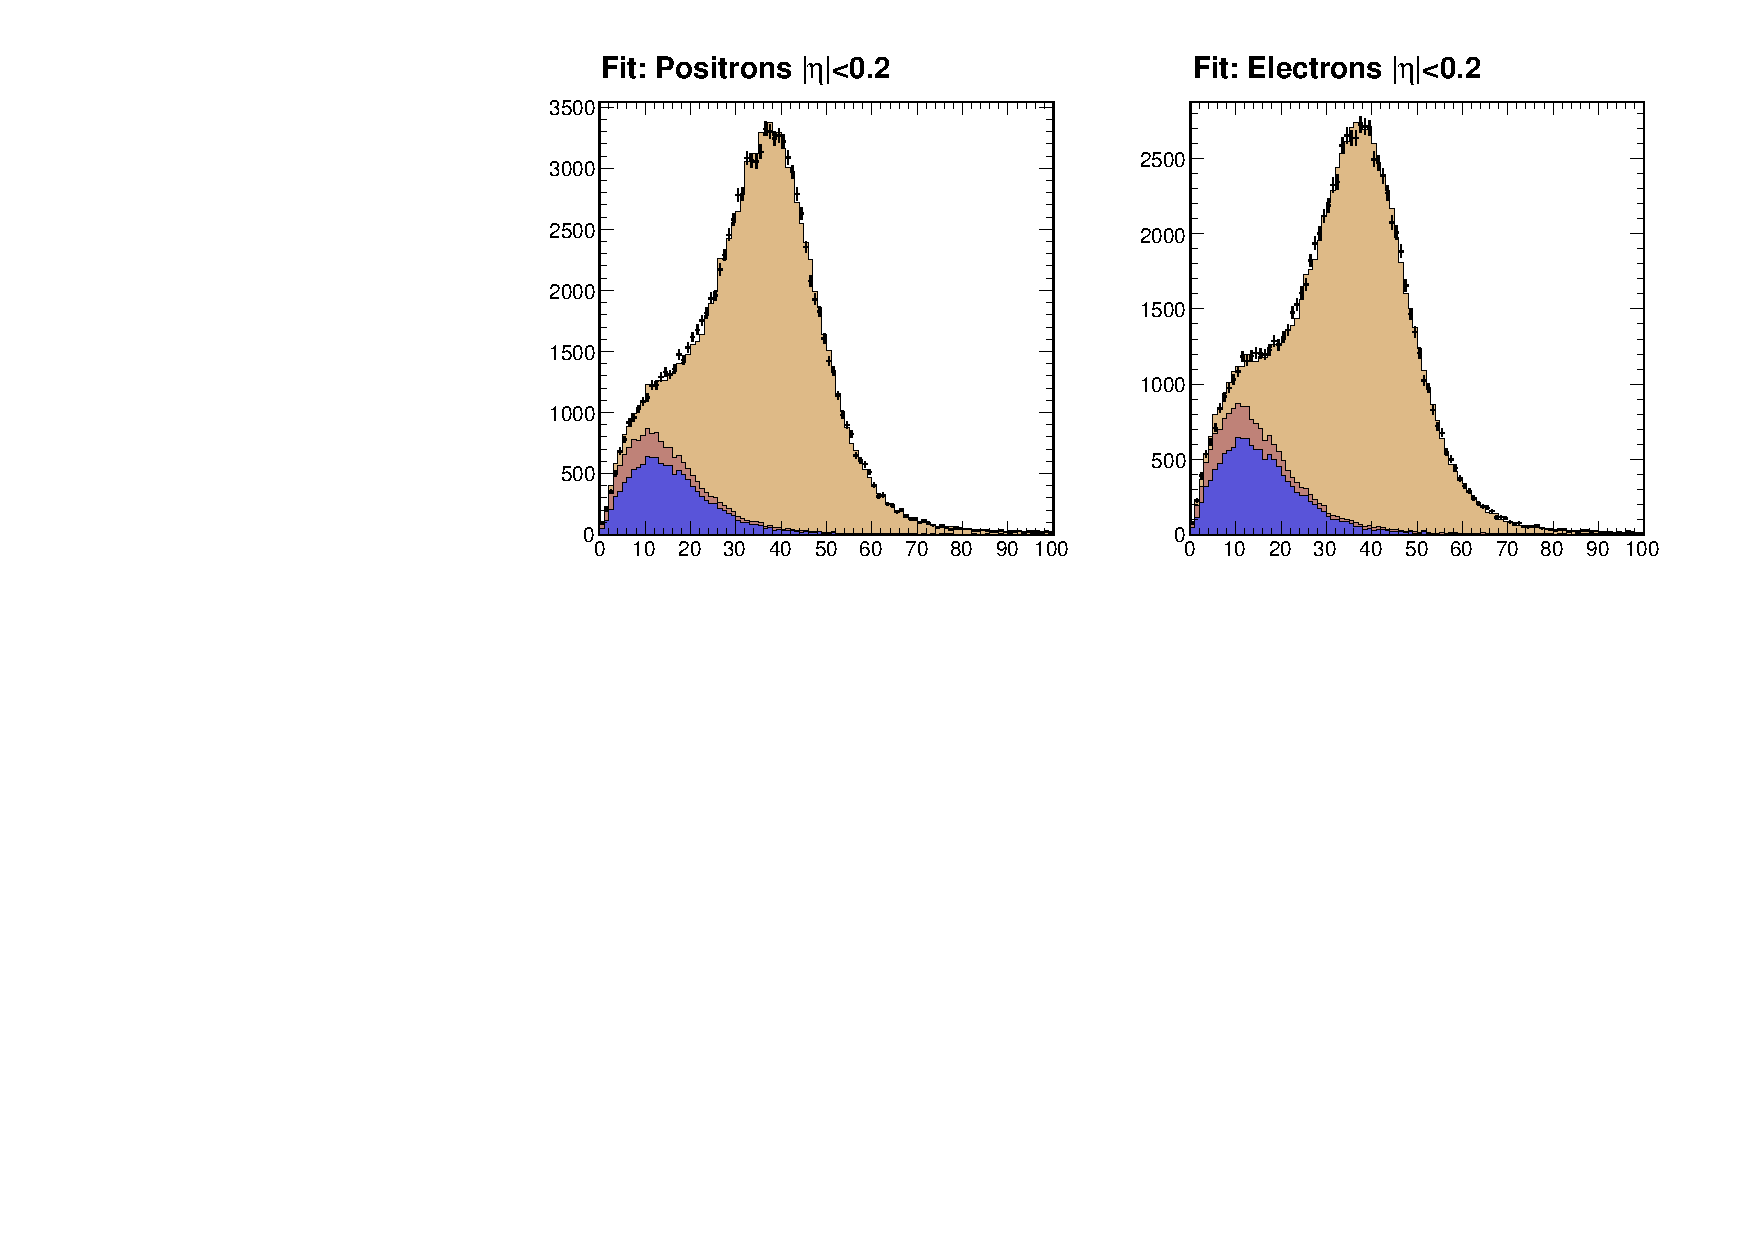
\includegraphics[width=0.95\textwidth]{data_0.pdf} \\
    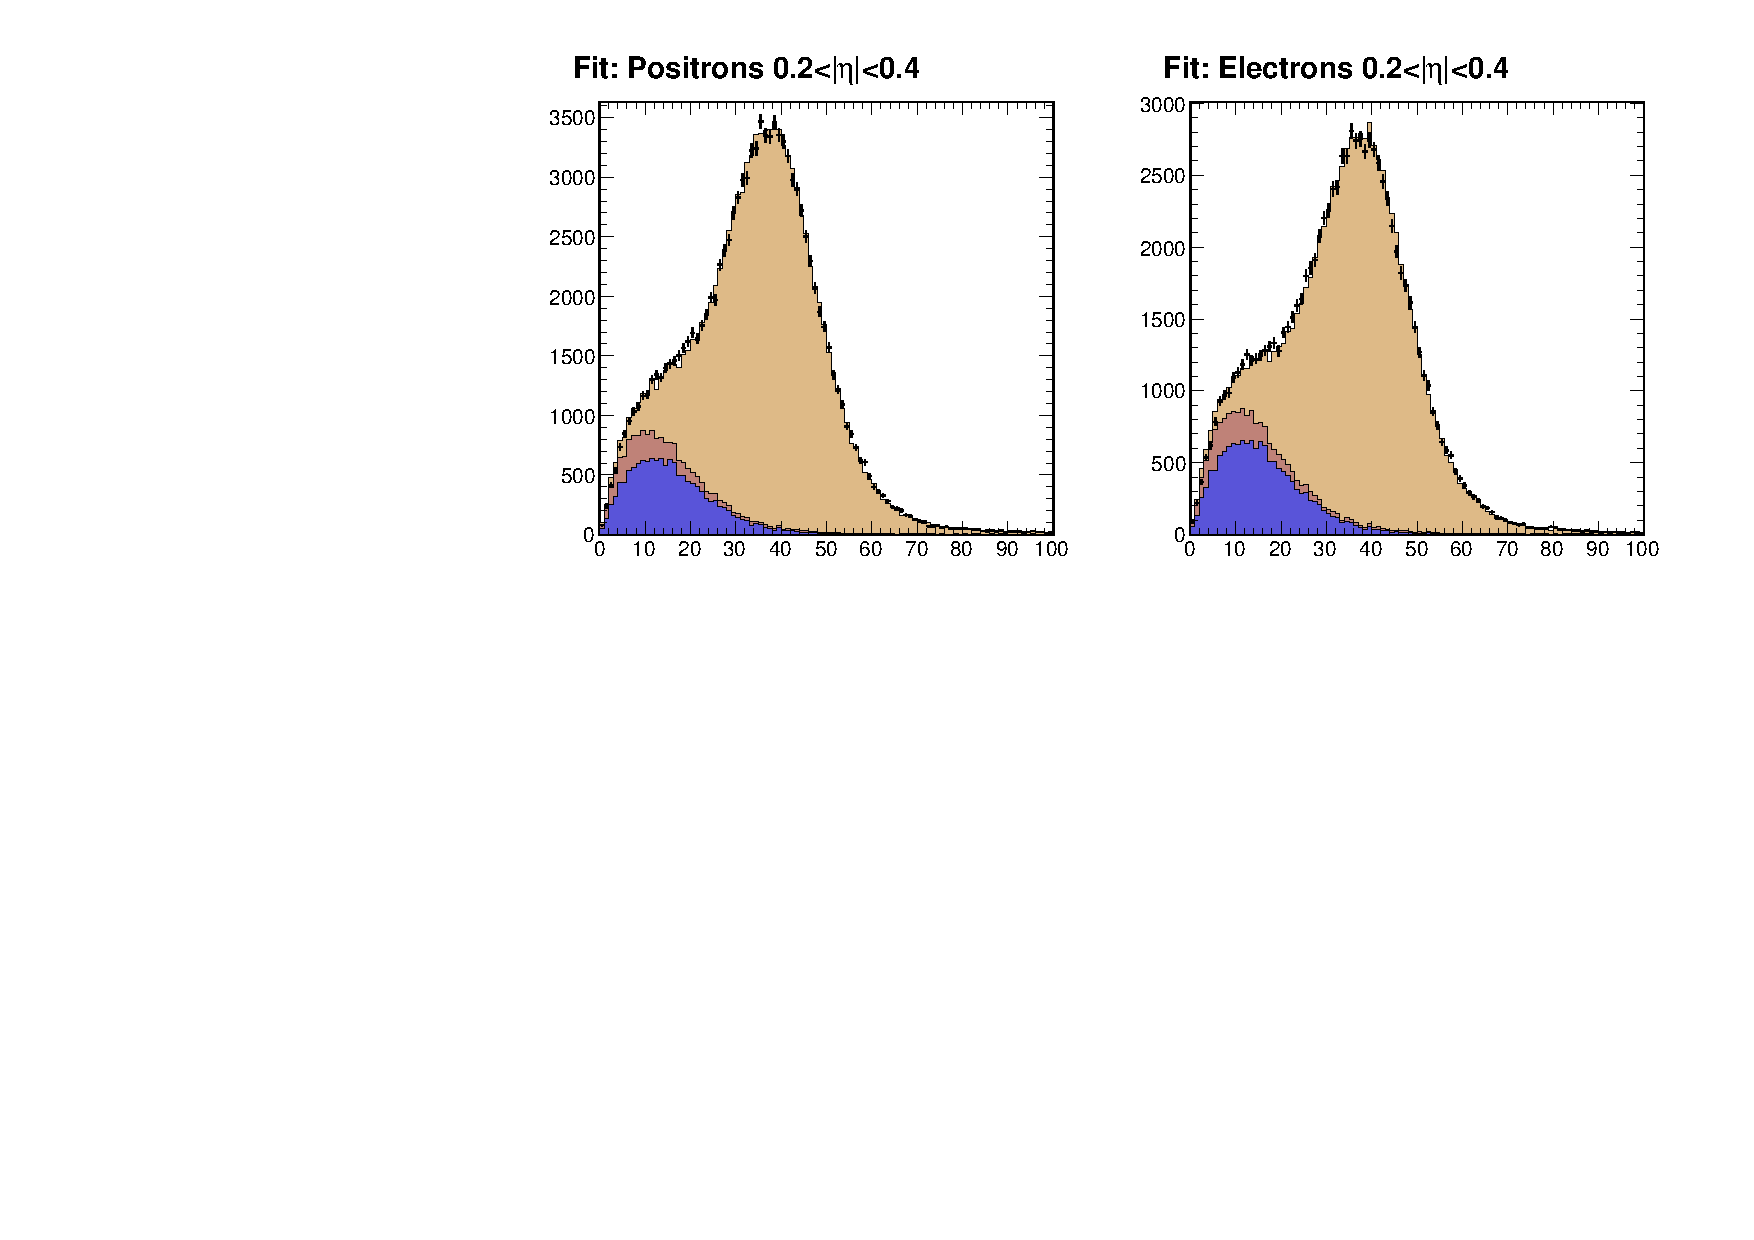
\includegraphics[width=0.95\textwidth]{data_1.pdf} \\
    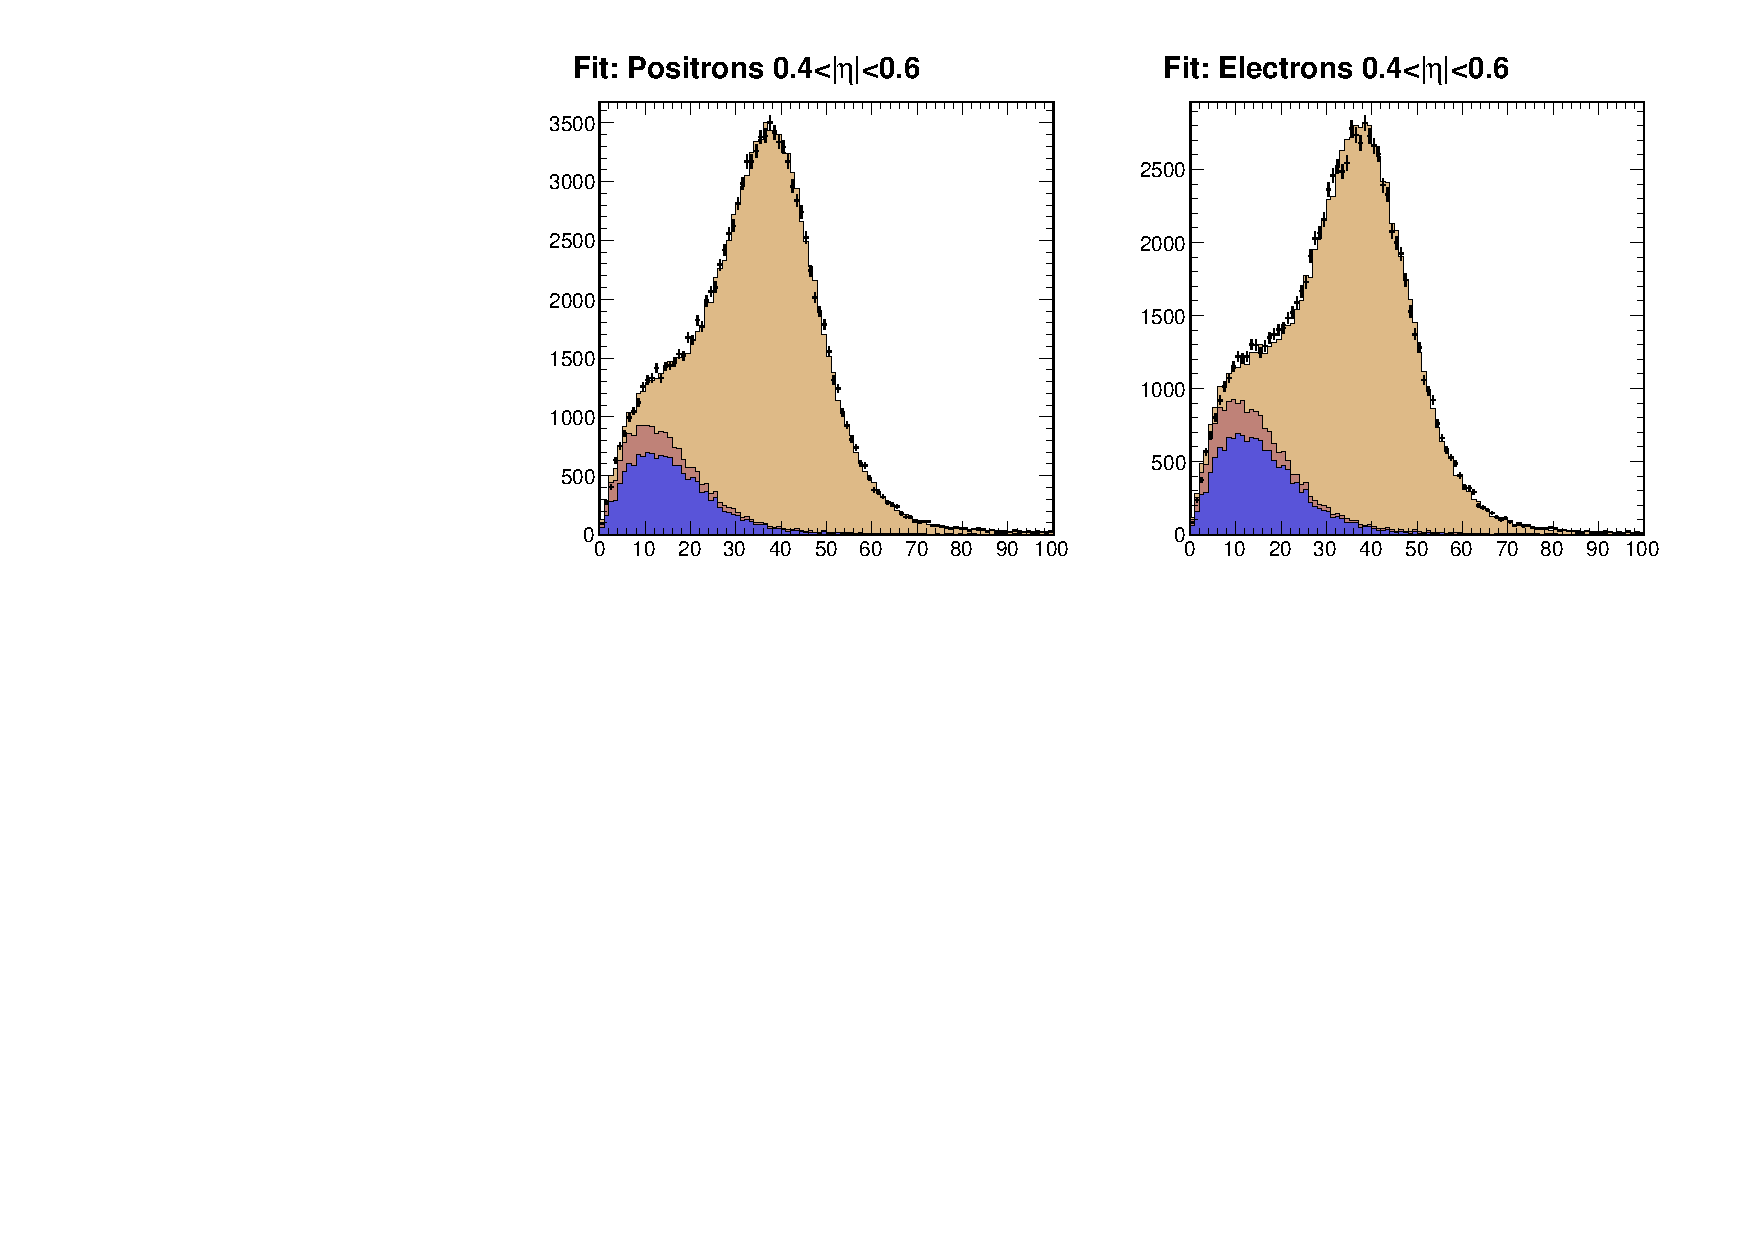
\includegraphics[width=0.95\textwidth]{data_2.pdf}
 \caption{  \label{fig:data1} The fit to \MET\ for eta bins 1,2 and 3.}
  \end{center}
\end{figure}

\begin{figure}
  \begin{center}
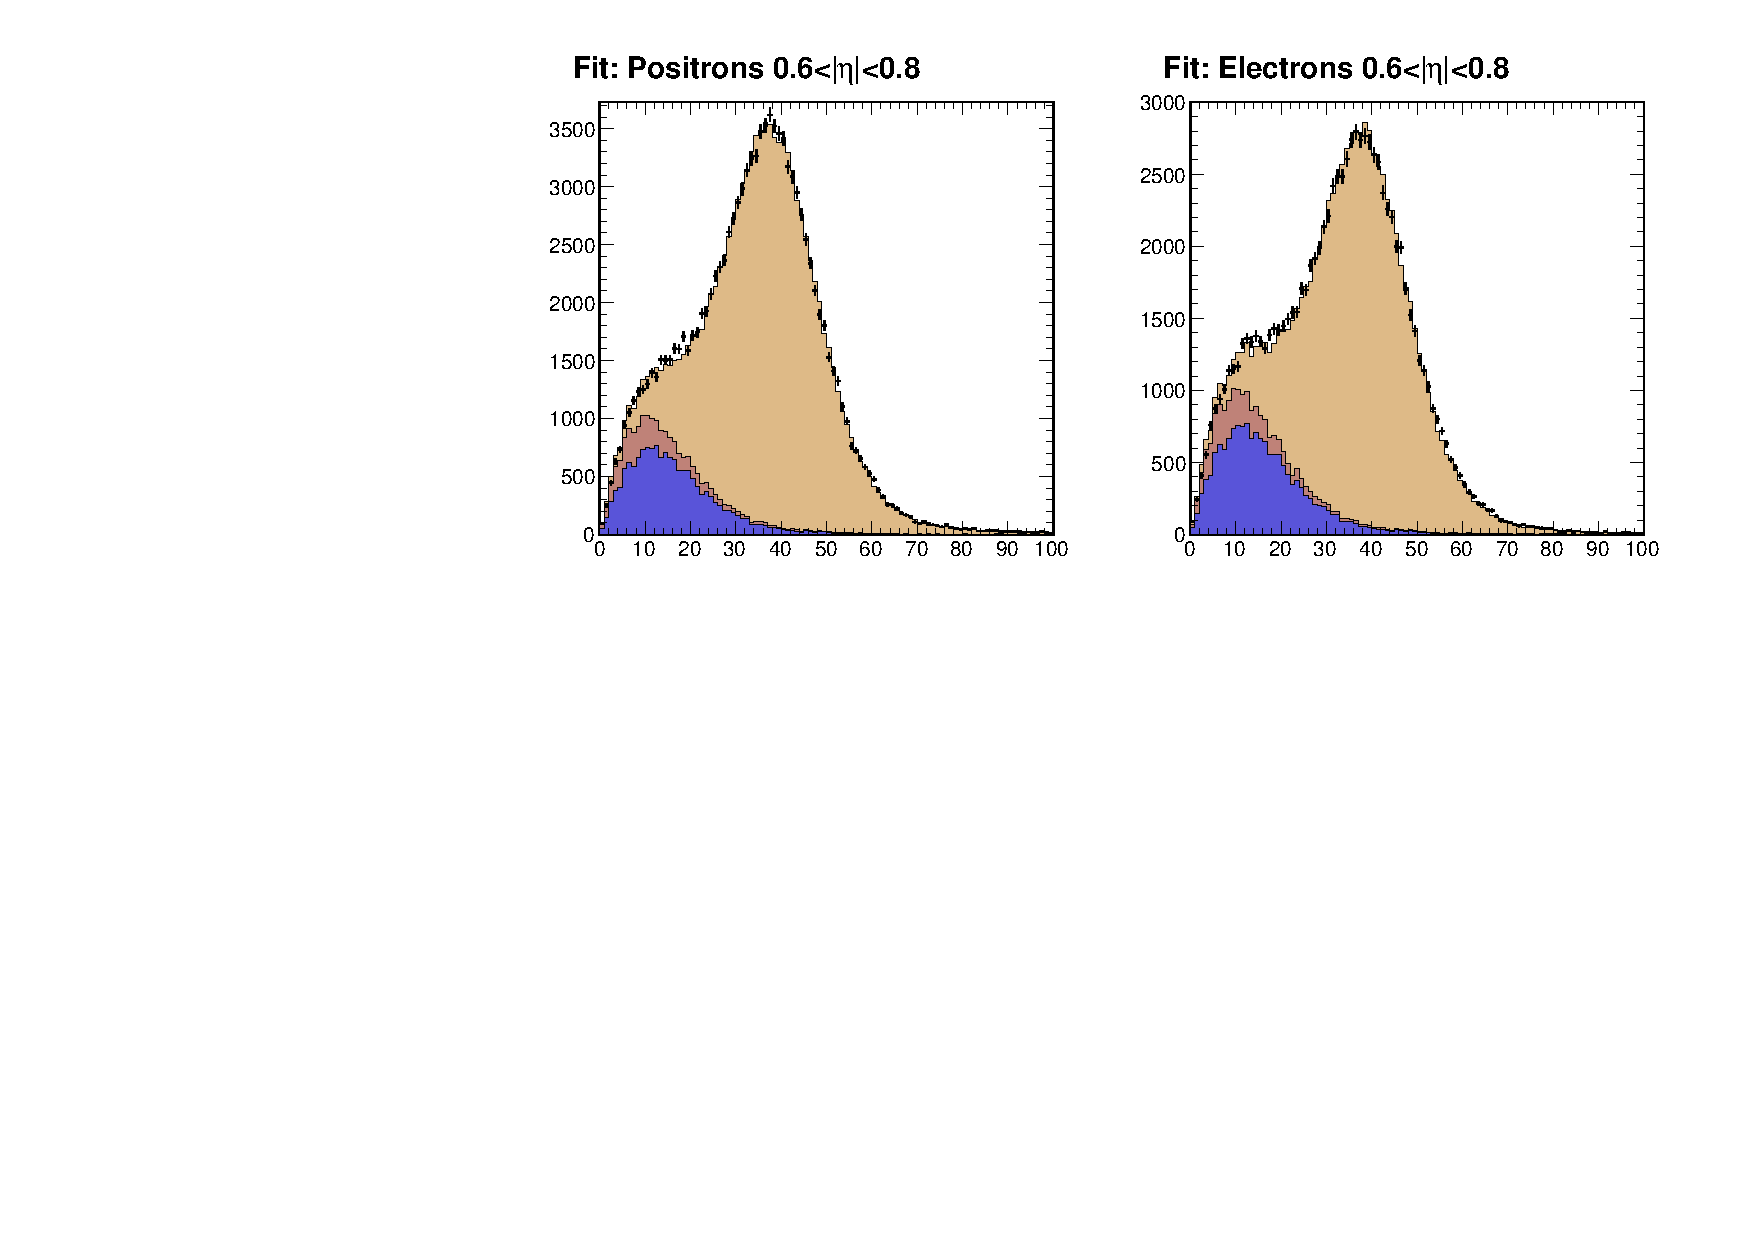
\includegraphics[width=0.95\textwidth]{data_3.pdf} \\
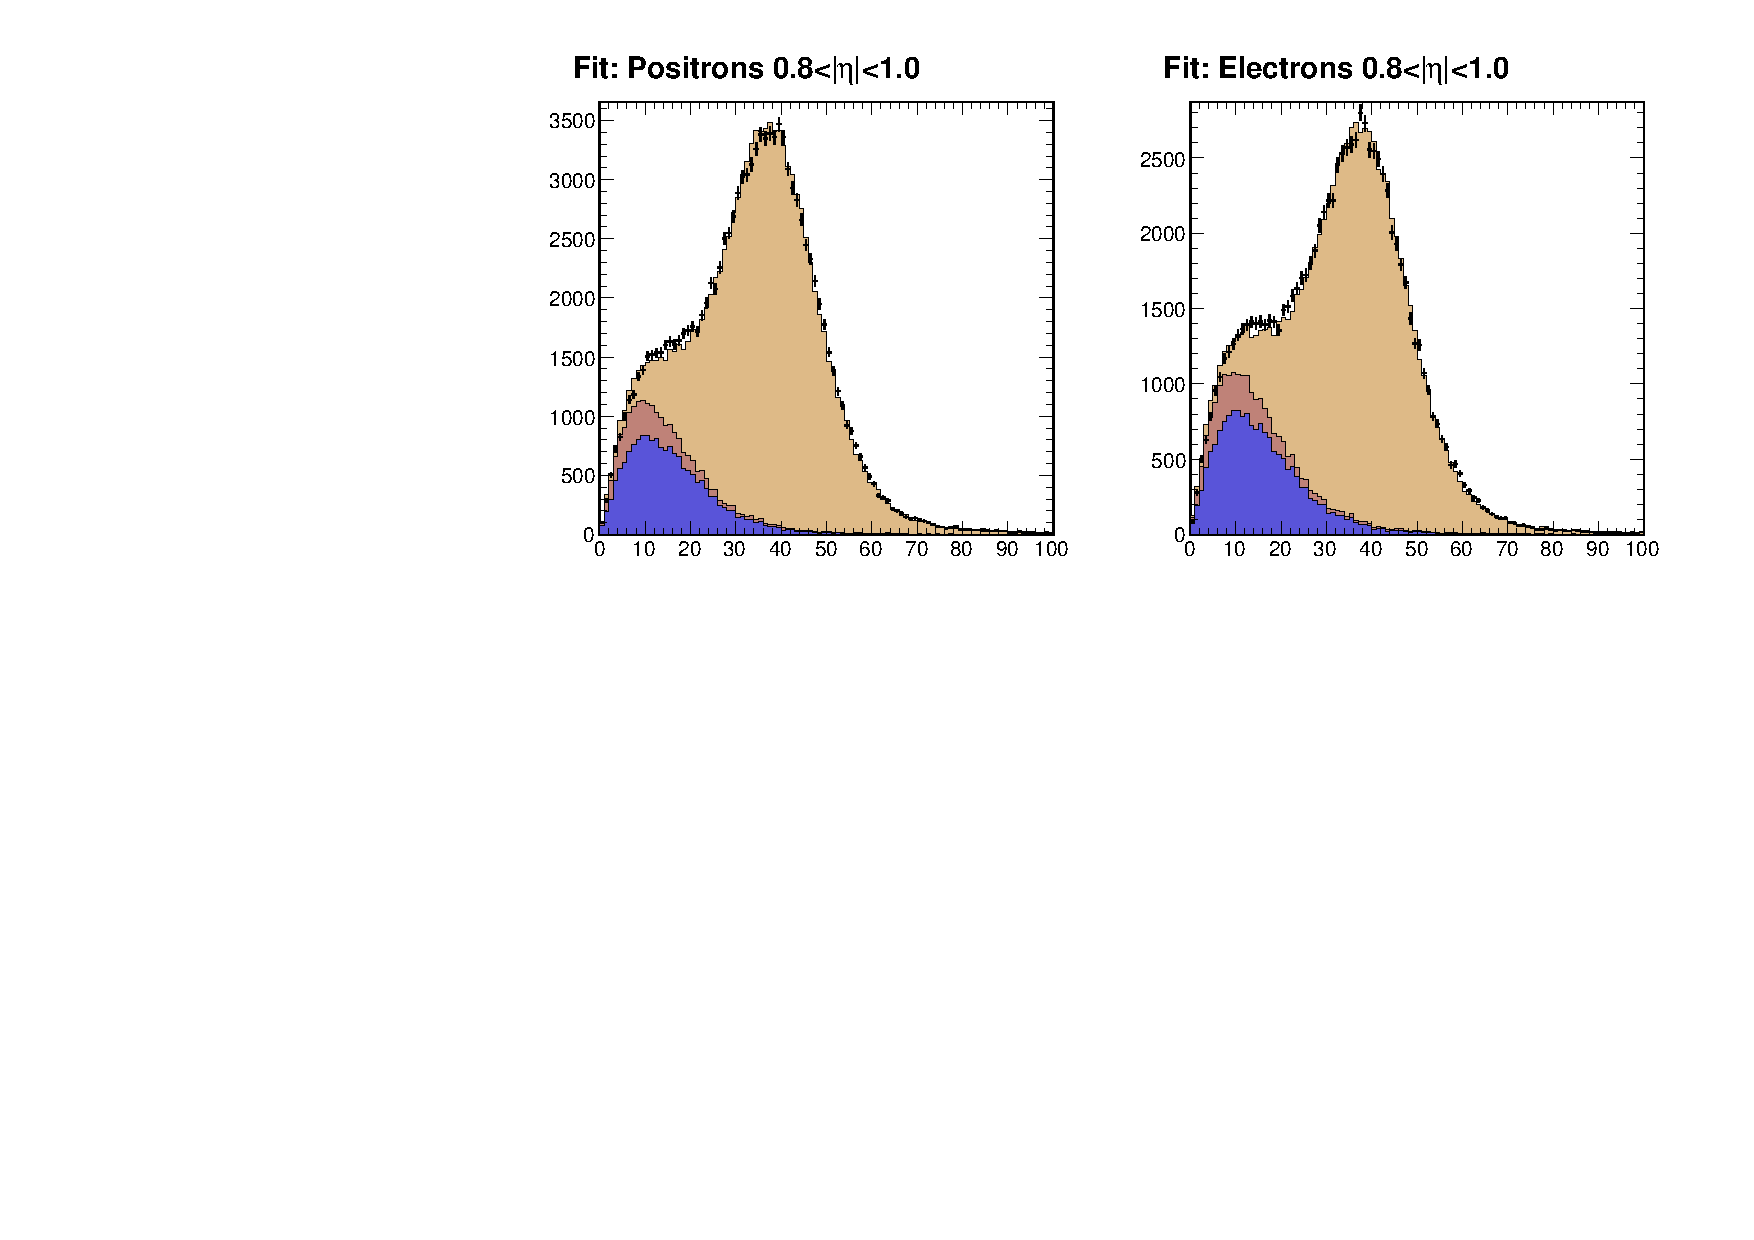
\includegraphics[width=0.95\textwidth]{data_4.pdf} \\
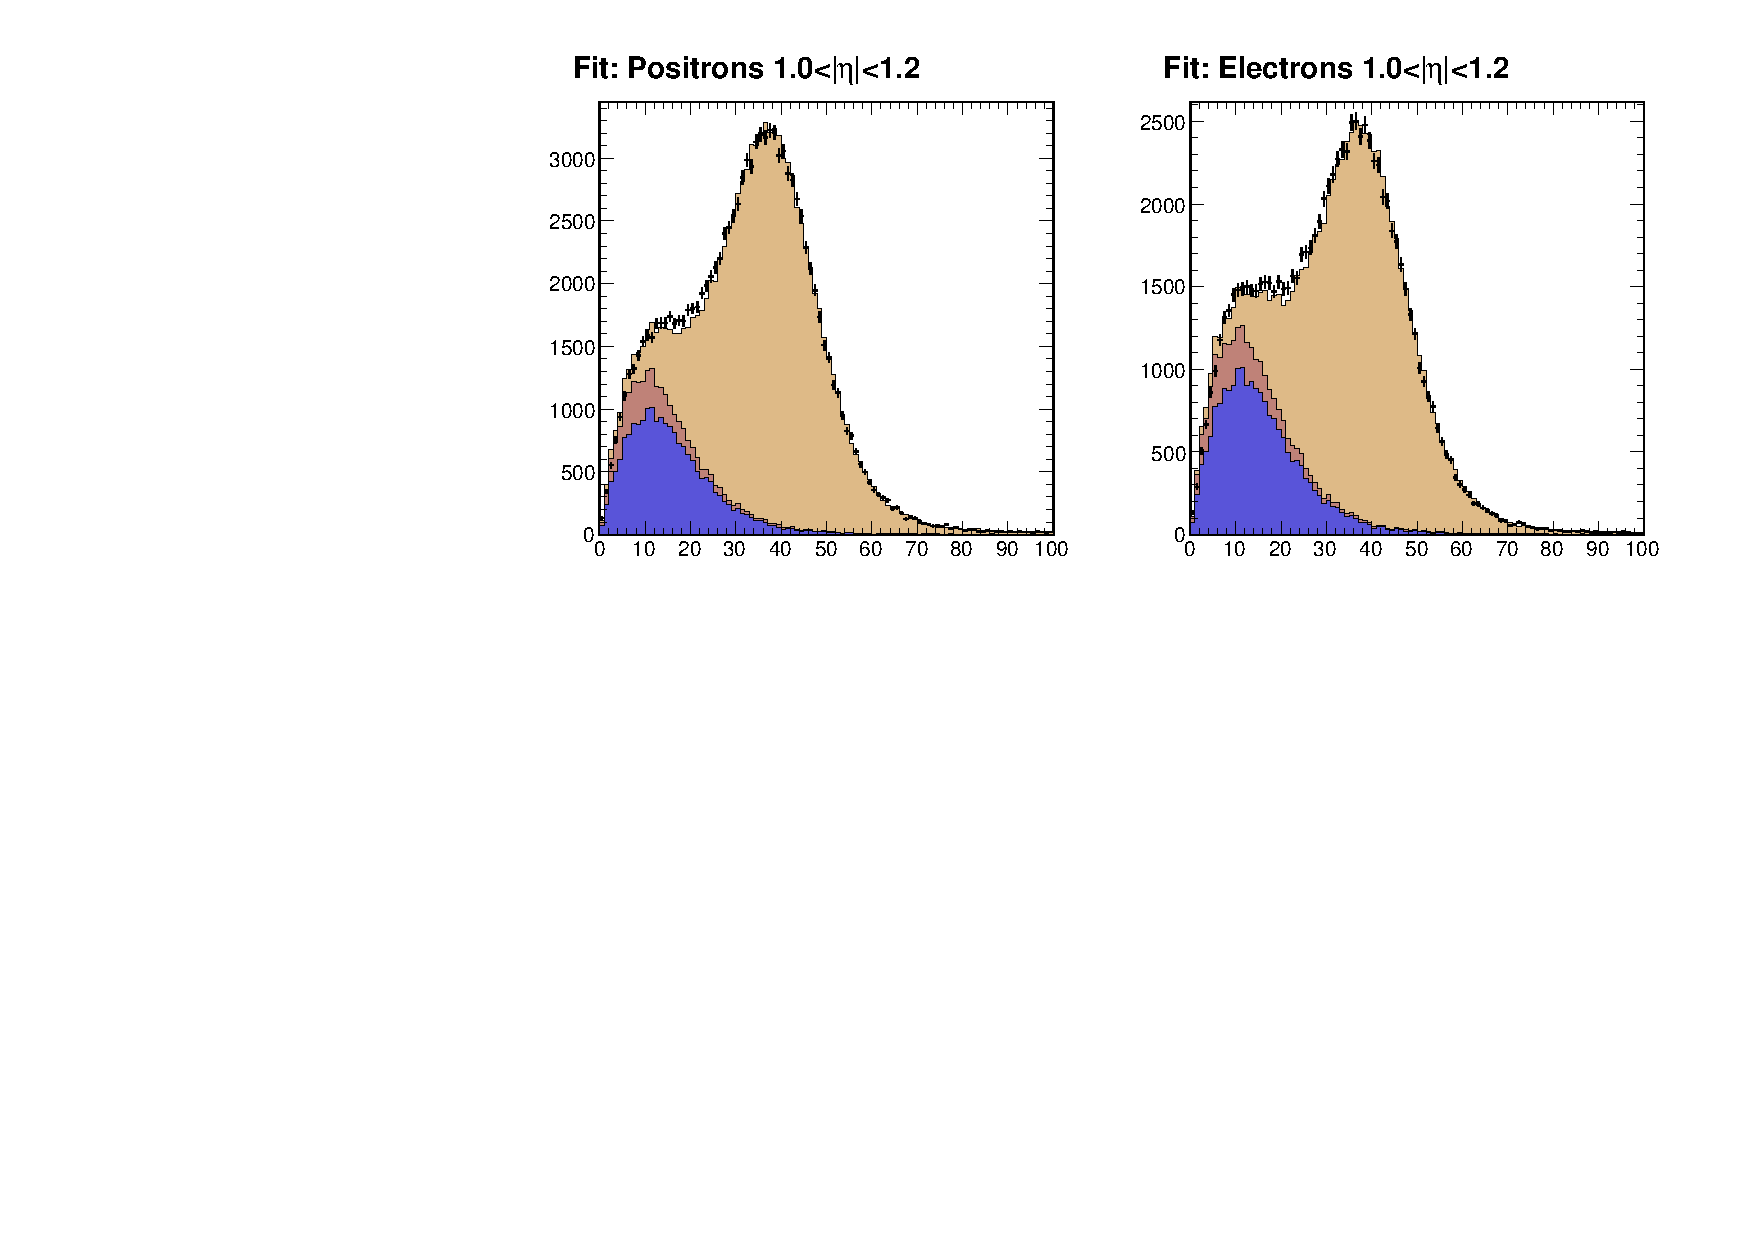
\includegraphics[width=0.95\textwidth]{data_5.pdf}
 \caption{  \label{fig:data2} The fit to \MET\ for eta bins 4,5 and 6.}
  \end{center}
\end{figure}

\begin{figure}
  \begin{center}
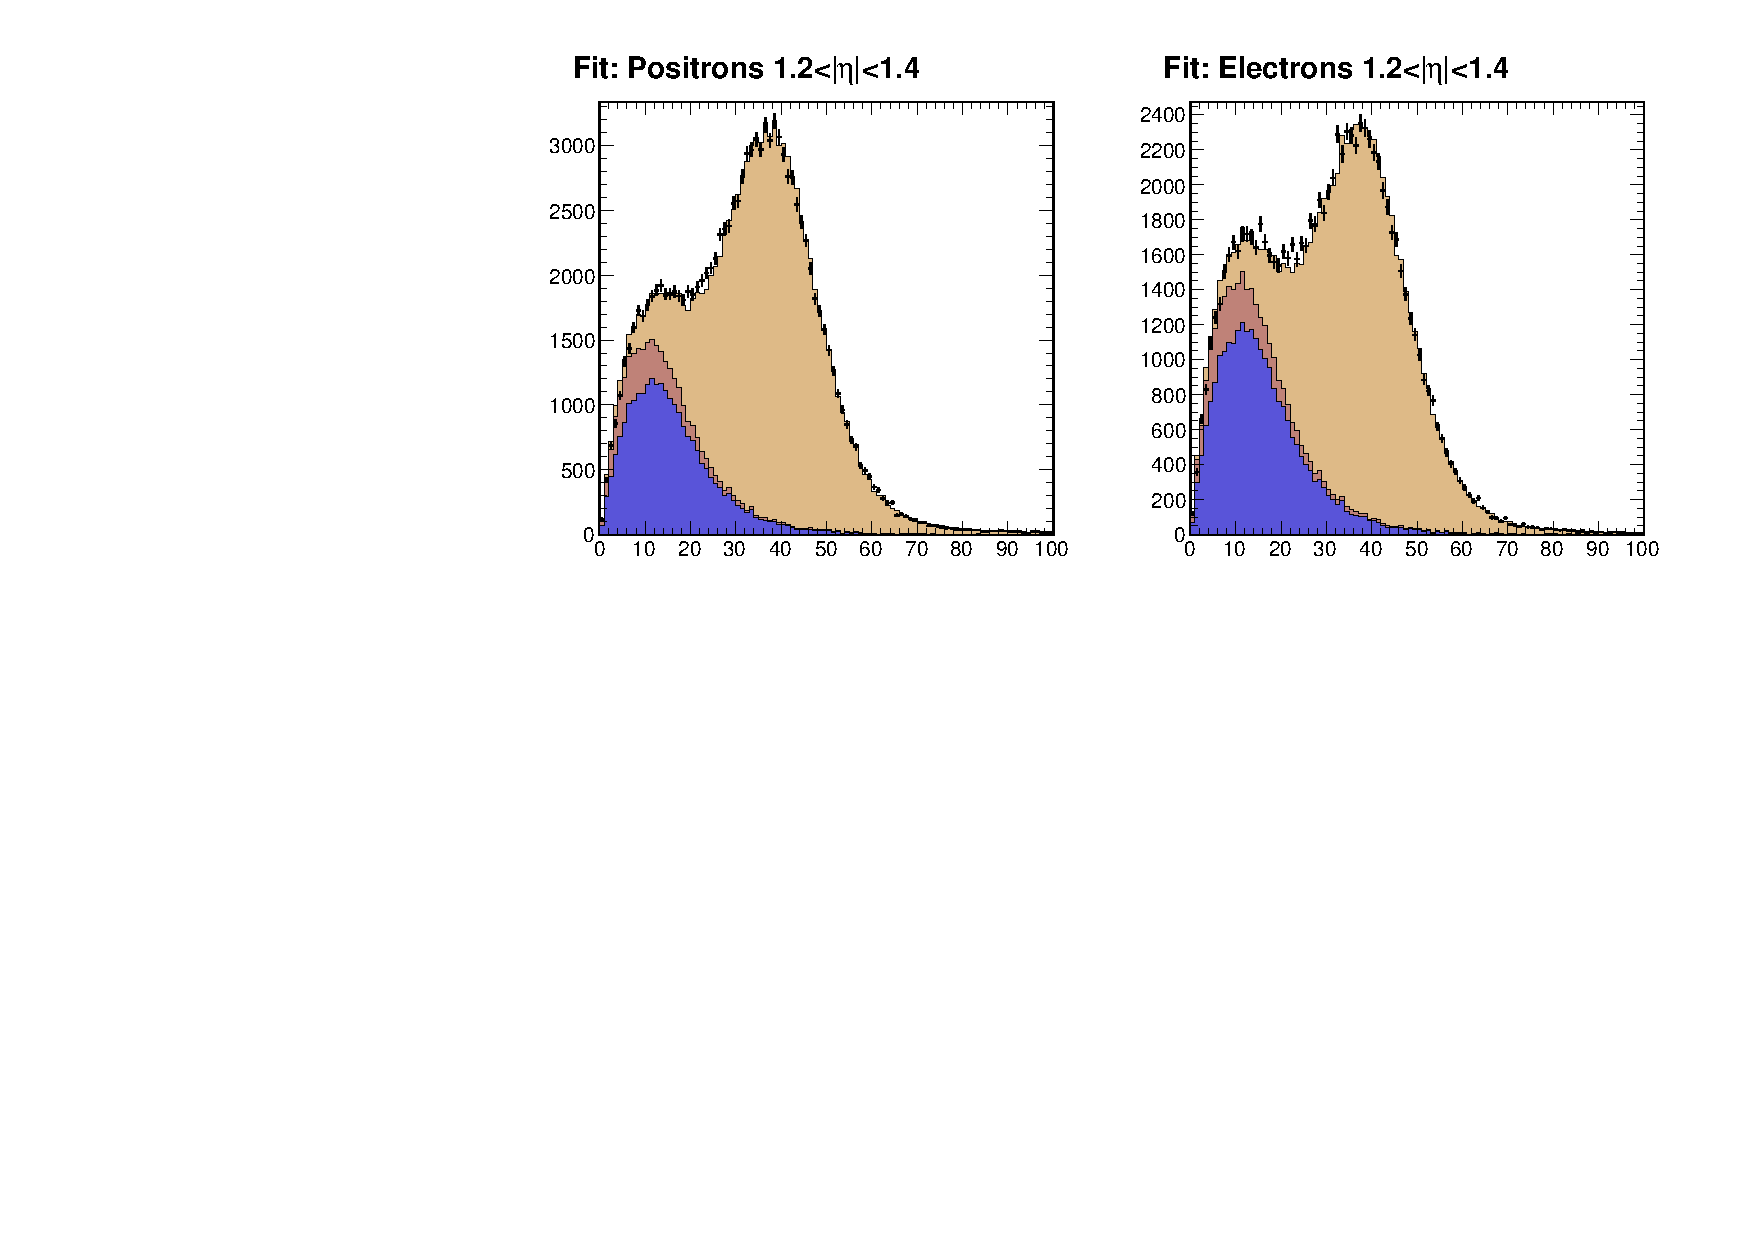
\includegraphics[width=0.95\textwidth]{data_6.pdf} \\
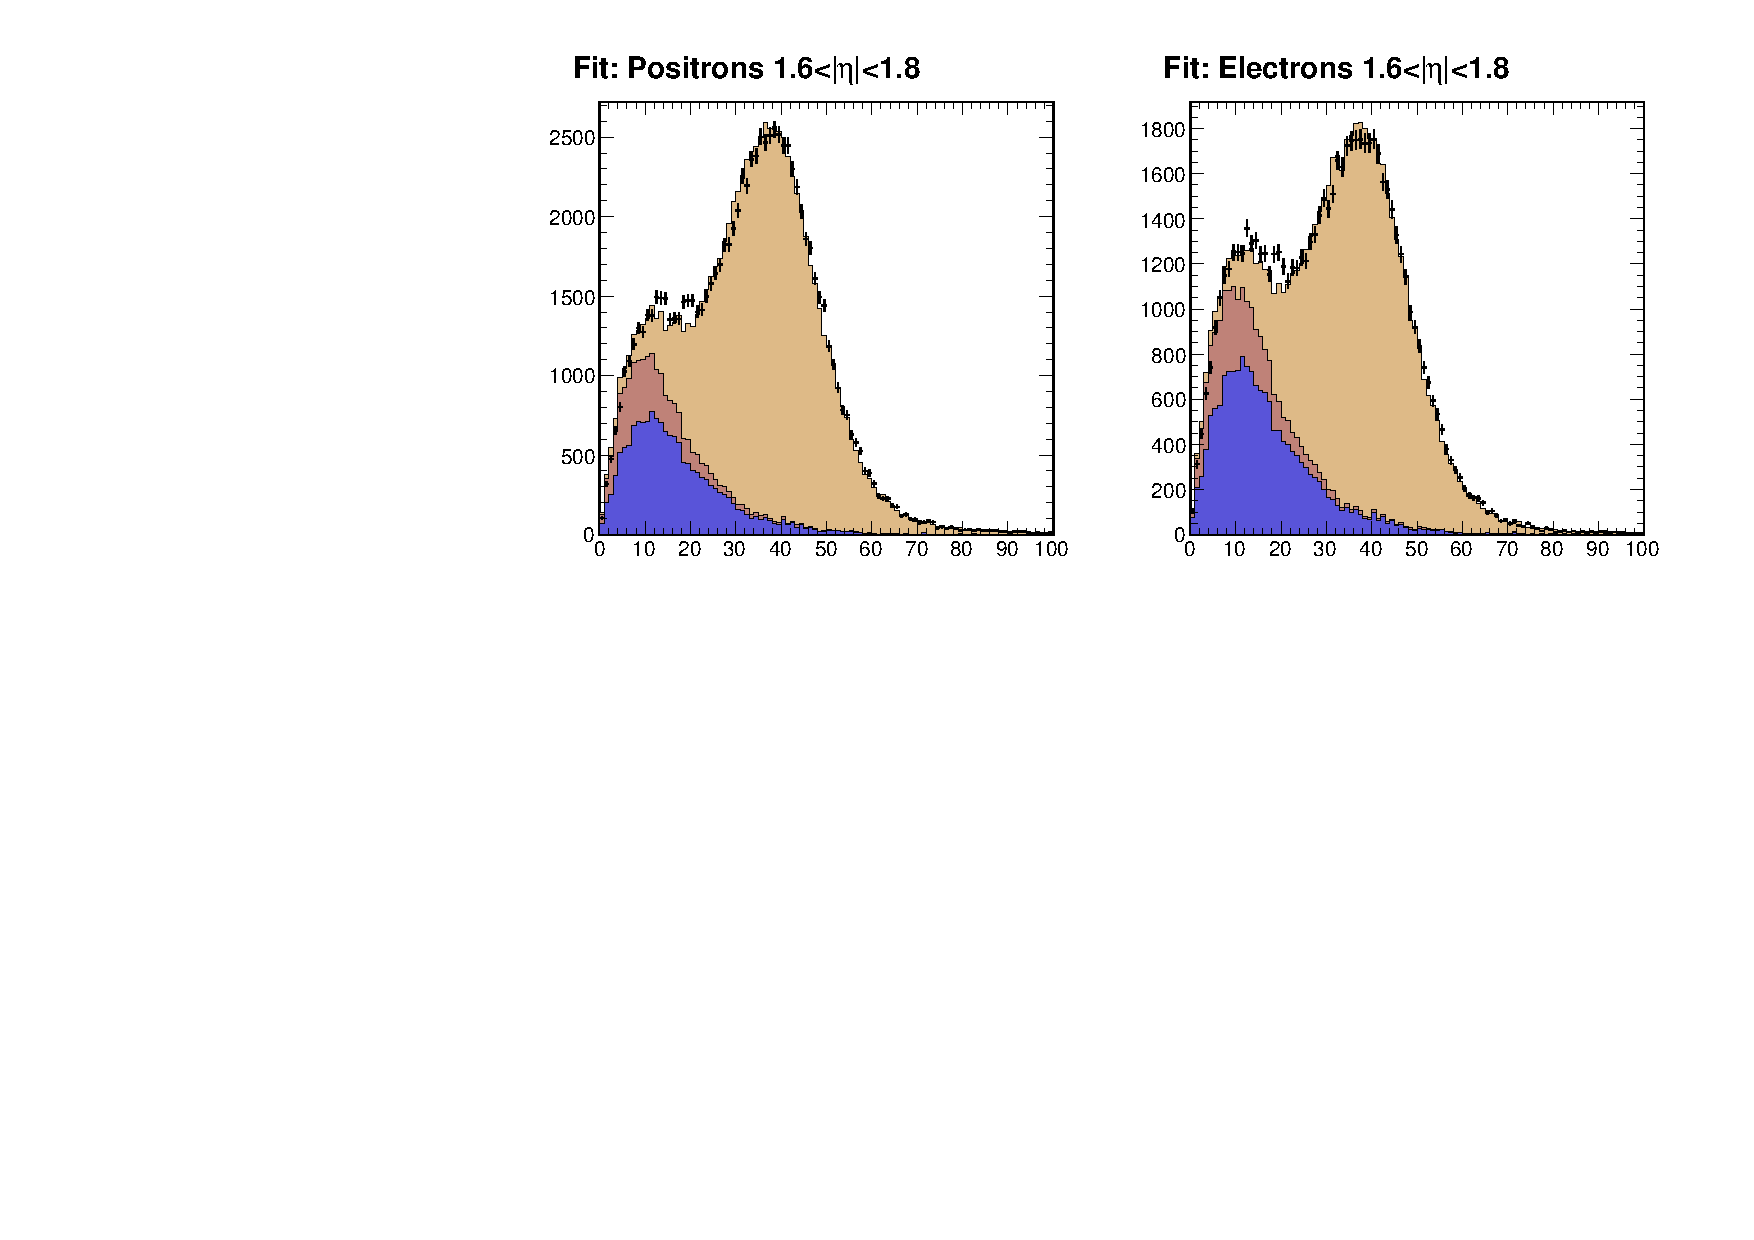
\includegraphics[width=0.95\textwidth]{data_7.pdf} \\
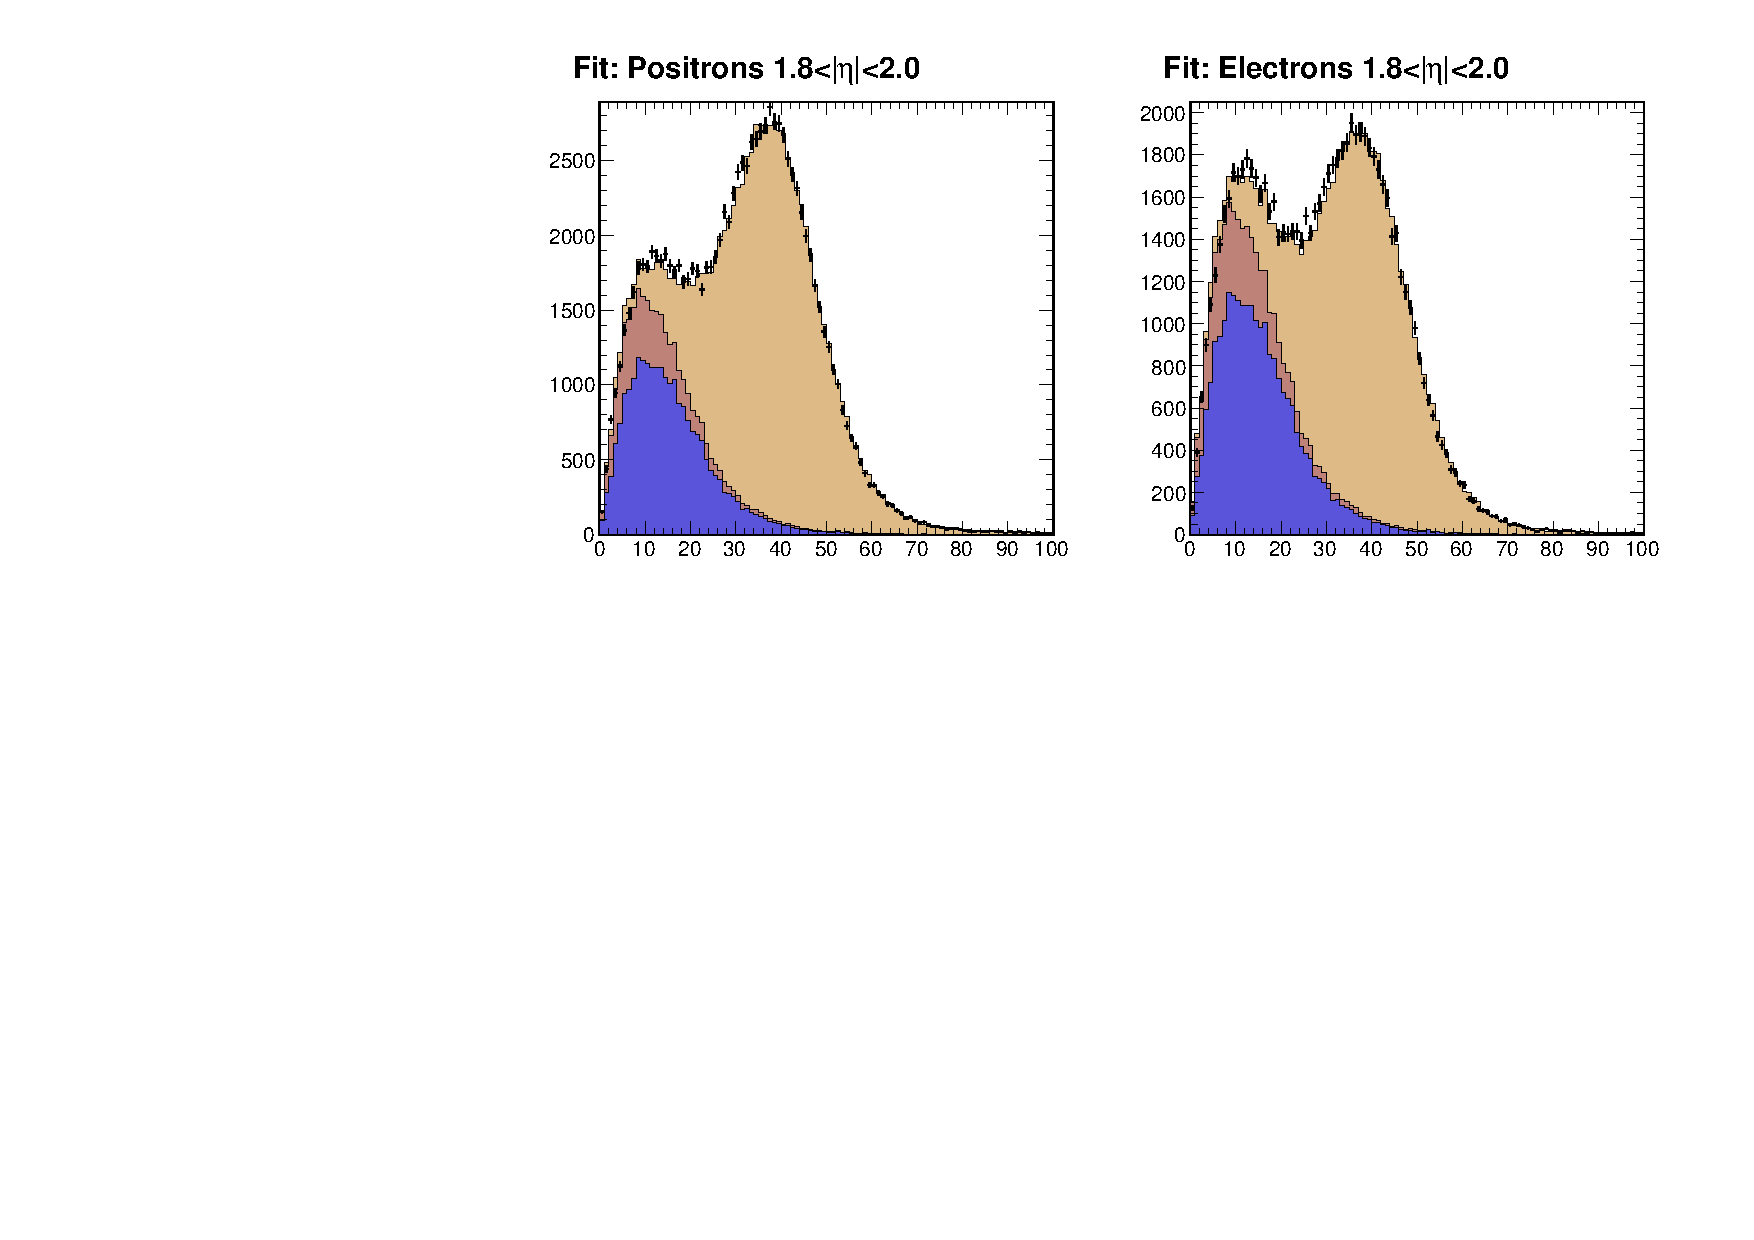
\includegraphics[width=0.95\textwidth]{data_8.pdf}
 \caption{  \label{fig:data3} The fit to \MET\ for eta bins 7,8 and 9.}
  \end{center}
\end{figure}

\begin{figure}
  \begin{center}
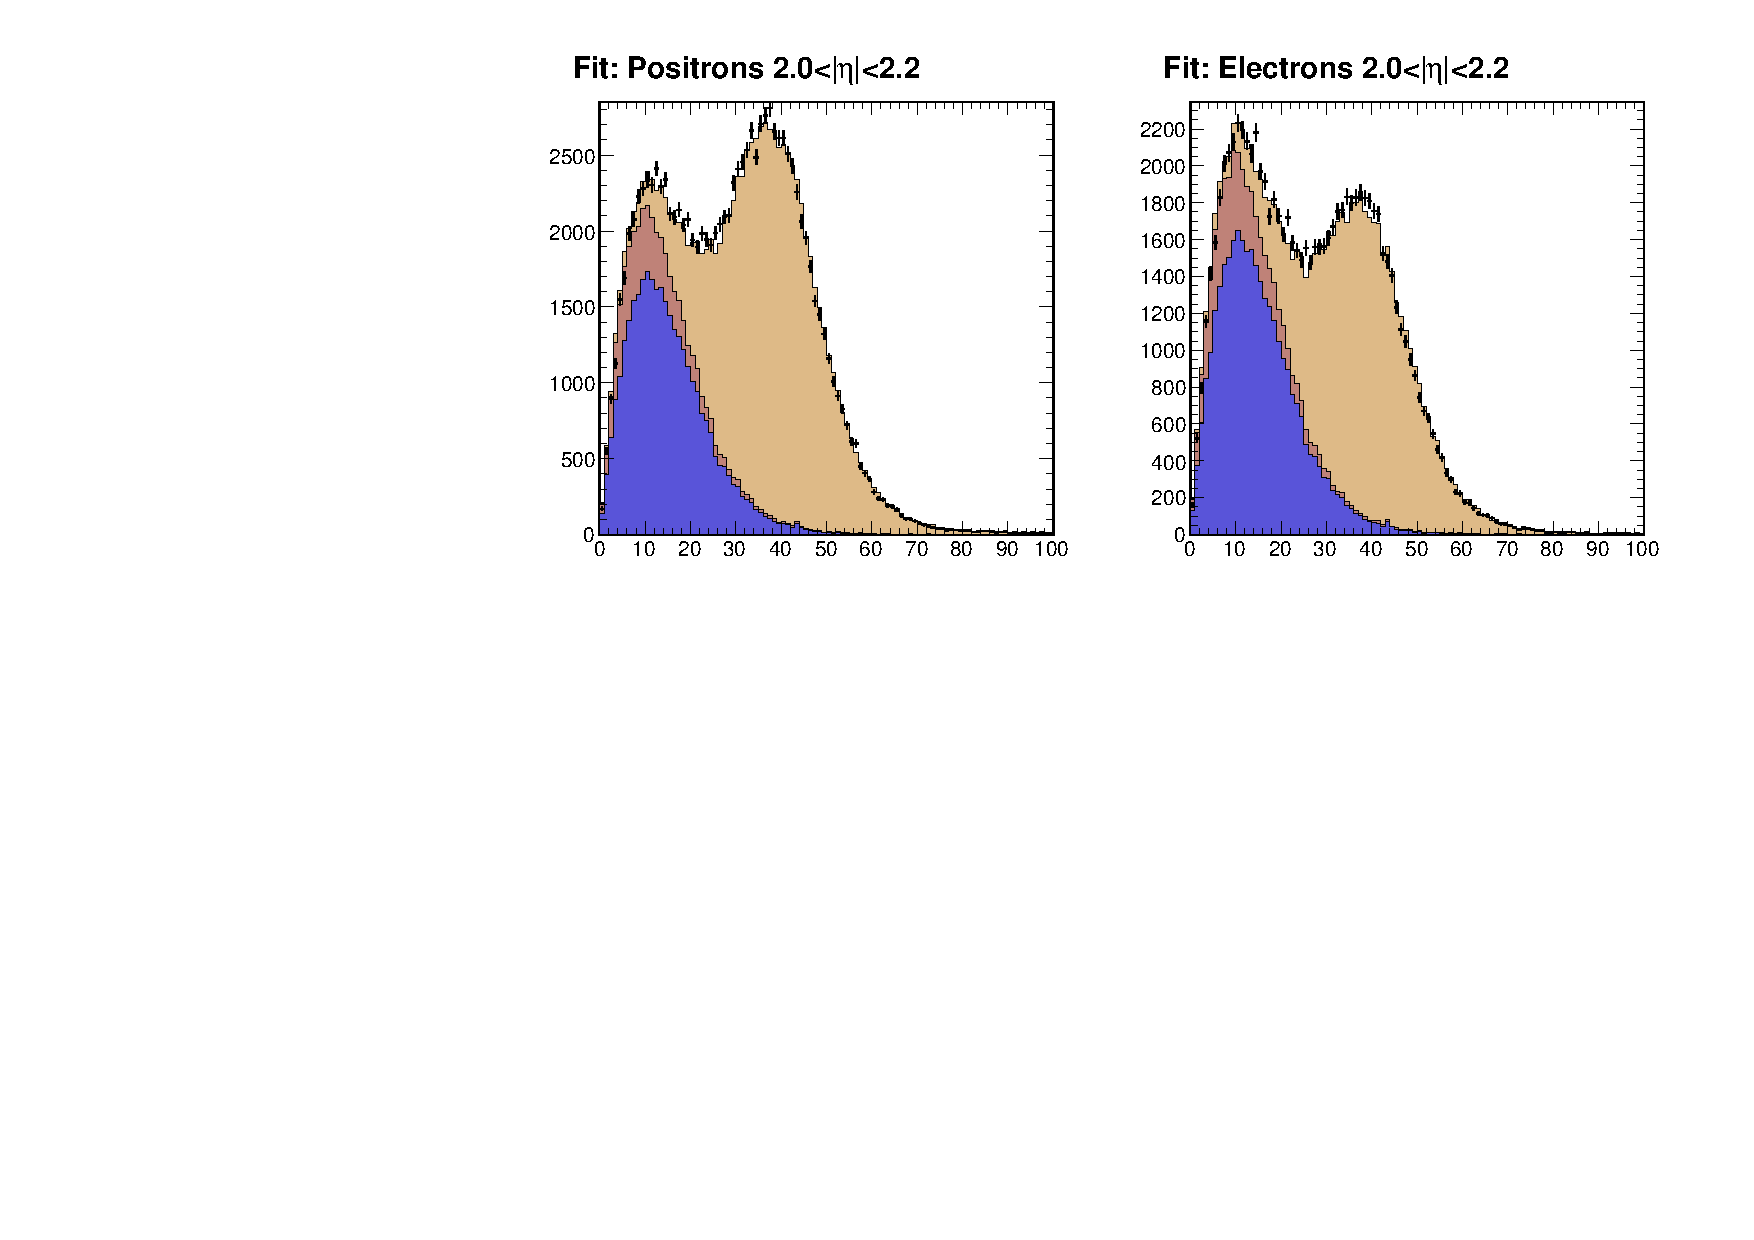
\includegraphics[width=0.95\textwidth]{data_9.pdf} \\
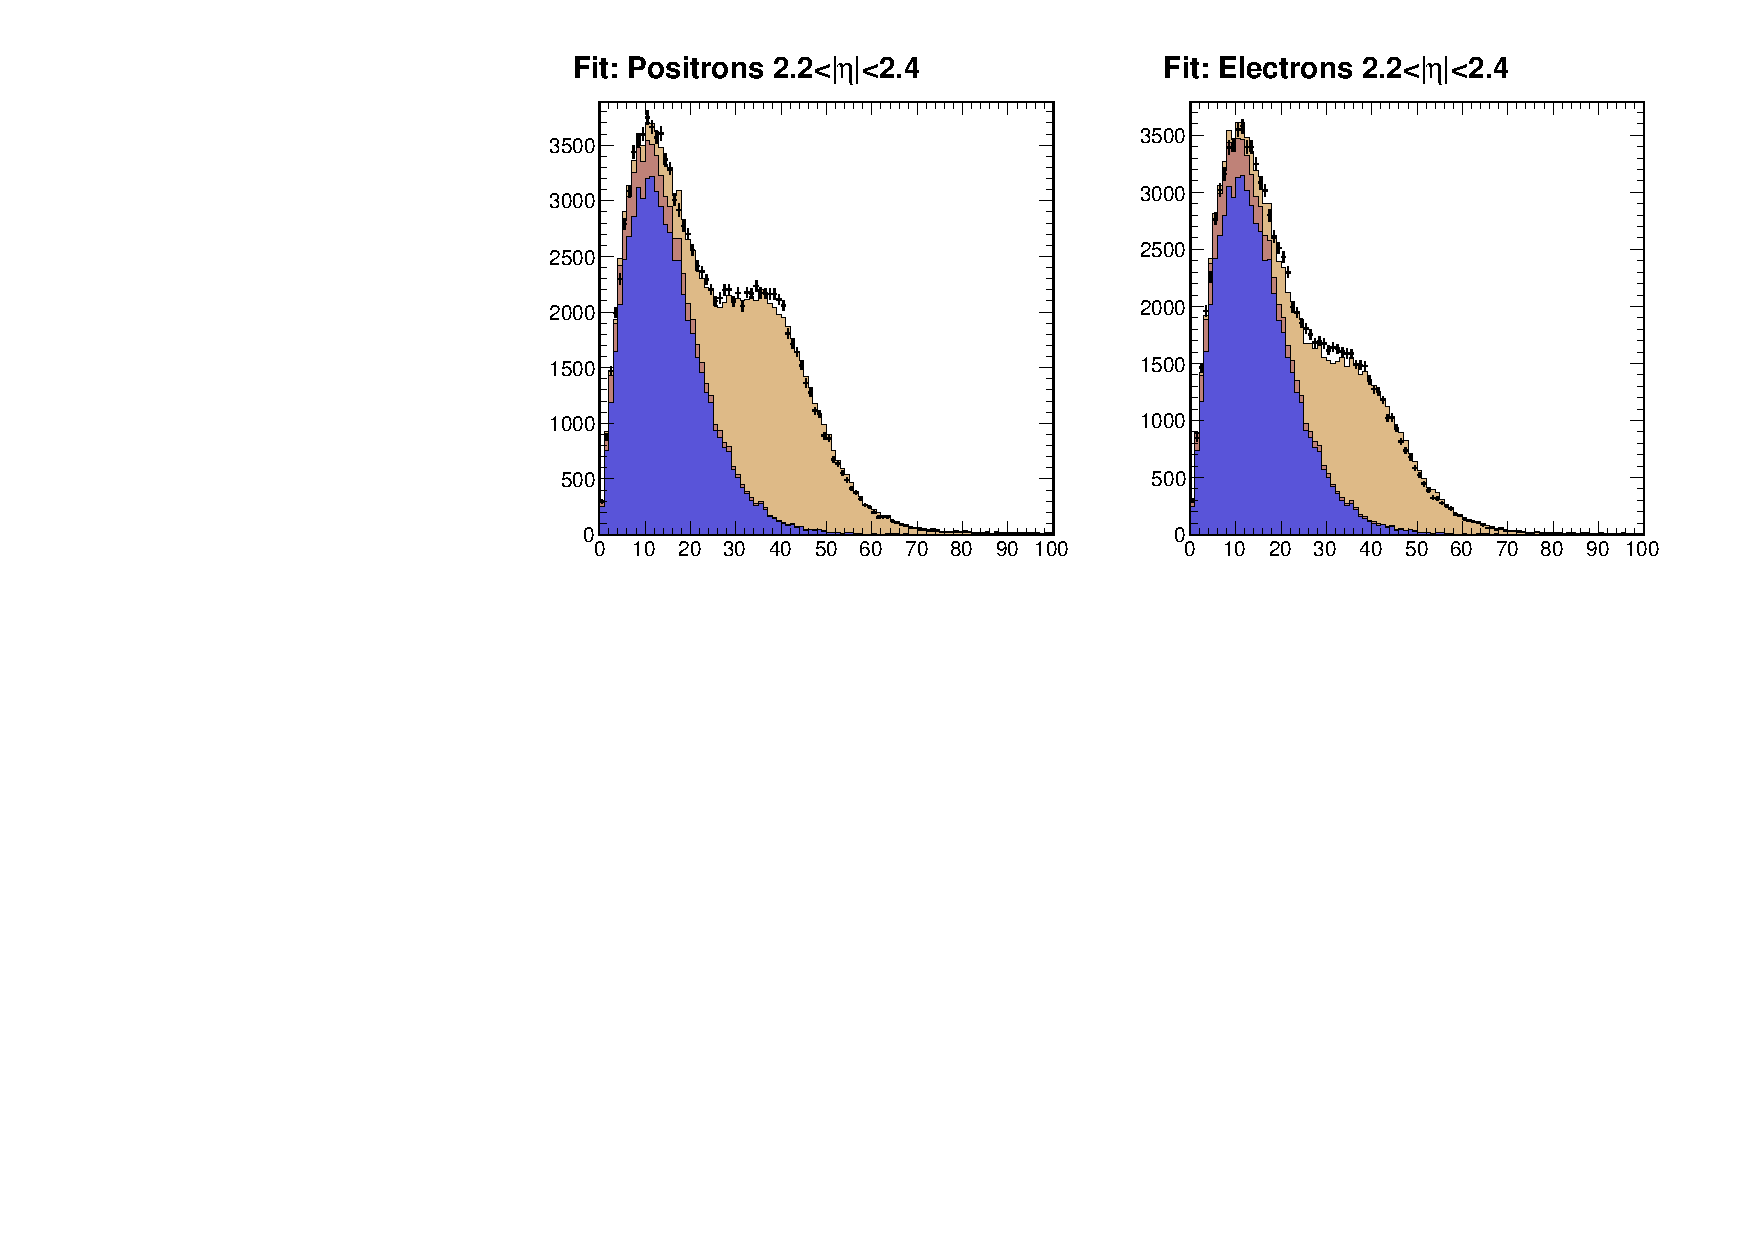
\includegraphics[width=0.95\textwidth]{data_10.pdf}
  \caption{  \label{fig:data4} The fit to \MET\ for eta bins 10 and 11.}
   \end{center}
\end{figure}

\begin{table}[htb]
 \begin{center}
 \begin{tabular}{lcrrrr}
$|\eta|$ range &  Charge &  N$_{QCD}$     & N$_{W\rightarrow e \nu}$  & N$_{W\rightarrow \tau \nu}$ & KS probability \\
               &         & fitted events & fitted events            & fitted events               & of fit \\
 \hline

$0.0<| \eta |<0.2$ &  +& $12794.5 \pm 202.6$ &$89698.3\pm330.5$&$ 1264.0\pm4.7 $&0.999 \\
                   &  -& $12926.1 \pm 194.3$ &$72369.8\pm297.6$&$ 1060.5\pm4.7 $&0.999 \\ 
$0.2<| \eta |<0.4$ &  +& $13773.9 \pm 209.6$ &$93109.0\pm337.7$&$ 1284.3\pm4.7 $&0.999 \\
                   &  -& $14071.4 \pm 199.8$ &$74215.4\pm302.0$&$ 1140.6\pm4.6 $&0.999 \\ 
$0.4<| \eta |<0.6$ &  +& $14803.9 \pm 212.9$ &$93211.7\pm338.1$&$ 1264.0\pm4.6 $&0.999 \\
                   &  -& $14554.2 \pm 203.5$ &$74360.3\pm303.4$&$ 1058.2\pm4.3 $&0.872 \\ 
$0.6<| \eta |<0.8$ &  +& $15484.5 \pm 217.0$ &$94943.5\pm341.0$&$ 1403.0\pm5.0 $&0.999 \\
                   &  -& $15523.8 \pm 206.4$ &$73764.2\pm302.2$&$ 1091.9\pm4.5 $&0.971 \\ 
$0.8<| \eta |<1.0$ &  +& $17177.5 \pm 221.7$ &$92971.3\pm338.1$&$ 1281.7\pm4.7 $&0.950 \\
                   &  -& $16871.6 \pm 210.5$ &$71476.6\pm298.3$&$ 1052.5\pm4.4 $&0.958 \\ 
$1.0<| \eta |<1.2$ &  +& $20001.2 \pm 229.9$ &$86449.0\pm329.0$&$ 1156.7\pm4.4 $&0.770 \\
                   &  -& $19930.1 \pm 218.4$ &$64643.8\pm286.6$&$ 957.0\pm4.2 $&0.676 \\ 
$1.2<| \eta |<1.4$ &  +& $24214.9 \pm 243.7$ &$83718.6\pm326.6$&$ 1115.6\pm4.4 $&0.985 \\
                   &  -& $24425.4 \pm 233.0$ &$60683.8\pm281.4$&$ 860.8\pm4.0 $&0.857 \\ 
$1.6<| \eta |<1.8$ &  +& $15759.0 \pm 228.6$ &$68726.0\pm302.3$&$ 939.0\pm4.1 $&0.480 \\
                   &  -& $16093.2 \pm 220.1$ &$47154.5\pm256.2$&$ 710.0\pm3.9 $&0.797 \\ 
$1.8<| \eta |<2.0$ &  +& $23809.6 \pm 241.7$ &$73116.7\pm305.0$&$ 908.4\pm3.8 $&0.915 \\
                   &  -& $23135.2 \pm 234.7$ &$49577.2\pm257.0$&$ 751.8\pm3.9 $&0.416 \\ 
$2.0<| \eta |<2.2$ &  +& $33773.0 \pm 261.7$ &$69872.7\pm299.1$&$ 846.4\pm3.6 $&0.581 \\
                   &  -& $32104.6 \pm 253.1$ &$45913.9\pm248.8$&$ 655.5\pm3.6 $&0.575 \\ 
$2.2<| \eta |<2.4$ &  +& $61794.8 \pm 309.3$ &$52495.9\pm269.8$&$ 607.9\pm3.1 $&0.386 \\
                   &  -& $60449.1 \pm 306.6$ &$34746.0\pm228.7$&$ 530.8\pm3.5 $&0.274 \\ 
 \end{tabular}
 \caption{\label{tab:chi2}
 Number of QCD events from the fitting procedure $\pm$ fit statistical uncertainty (Second column);
   Number of signal events  (Third column), Number of $W\rightarrow \tau \nu$ events (Fourth column),
 Kolmogorov-Smirnov probability (Fifth column).
 The quoted uncertainty for N$_{W\rightarrow e \nu}$ and N$_{W\rightarrow \tau \nu}$
 is the statistical uncertainty assigned to N$_{sig+EWK}$
 rescaled by the expected contribution of signal and $W\rightarrow \tau \nu$ in the signal+EWK template}
 \end{center}
\end{table}

\begin{table}[htb]
  \begin{center}
    \begin{tabular}{lc}
    $|\eta|$ range & $\mathcal{A}_{exp} (\times 10^{-3})$\\
    \hline
    $0.0<|\eta|<0.4$ & 106.9 $\pm$ 2.7\\
    $0.2<|\eta|<0.4$ & 112.9 $\pm$ 2.7\\
    $0.4<|\eta|<0.6$ & 112.5 $\pm$ 2.7\\
    $0.6<|\eta|<0.8$ & 125.5 $\pm$ 2.7\\
    $0.8<|\eta|<1.0$ & 130.7 $\pm$ 2.7\\
    $1.0<|\eta|<1.2$ & 144.3 $\pm$ 2.9\\
    $1.2<|\eta|<1.4$ & 159.5 $\pm$ 3.0 \\
    $1.6<|\eta|<1.8$ & 186.1 $\pm$ 3.4\\
    $1.8<|\eta|<2.0$ & 191.8 $\pm$ 3.2\\
    $2.0<|\eta|<2.2$ & 206.9 $\pm$ 3.3\\
    $2.2<|\eta|<2.4$ & 203.4 $\pm$ 4.1\\
    \end{tabular}
  \caption{\label{tab:uncorRes}Uncorrected values ($\times 10^{-3}$) of the
  charge asymmetry  for an integrated luminosity of \unit{840}{\invpb}. }
  \end{center}
\end{table}

\section{Corrections}
\todo[inline]{introduction to corrections}

\subsection{Relative Efficiency}
\todo[inline]{Relative efficiency systematic}


\begin{table}[htb]
\begin{center}
\begin{tabular}{lcrrrr}
$|\eta|$ range & Charge & $\epsilon_{GSF}$ &$\epsilon_{ID}$&$\epsilon_{HLT}$& R\\
\hline
$0.0<| \eta |<0.2$ &+& 98.5$\pm$0.2 &83.6$\pm$0.4 &97.9$\pm$0.2 &1.003$\pm$0.009\\
                   &-& 98.4$\pm$0.2 &83.5$\pm$0.5 &97.8$\pm$0.2 & \\
$0.2<| \eta |<0.4$ &+& 98.9$\pm$0.2 &82.6$\pm$0.5 &97.9$\pm$0.2 & 0.998$\pm$0.009\\
                   &-& 98.8$\pm$0.2 &82.8$\pm$0.5 &98.0$\pm$0.2 & \\
$0.4<| \eta |<0.6$ &+& 98.9$\pm$0.2&83.6$\pm$0.5 &98.1$\pm$0.2 & 0.995$\pm$0.009\\
                   &-& 99.0$\pm$0.2 &84.1$\pm$0.5 &97.9$\pm$0.2 & \\
$0.6<| \eta |<0.8$ &+& 98.7$\pm$0.2 &83.7$\pm$0.5 &98.4$\pm$0.2 & 0.999$\pm$0.009\\
                   &-& 98.7$\pm$0.2 &84.0$\pm$0.5&98.2$\pm$0.2 & \\
$0.8<| \eta |<1.0$ &+& 98.6$\pm$0.2 &84.3$\pm$0.5 &97.3$\pm$0.2 & 0.998$\pm$0.009\\
                   &-& 98.3$\pm$0.2 &84.4$\pm$0.5 &97.7$\pm$0.2 & \\
$1.0<| \eta |<1.2$ &+& 98.2$\pm$0.2 &82.6$\pm$0.5 &97.6$\pm$0.2 & 1.010$\pm$0.010\\
                   &-& 98.2$\pm$0.2 &81.7$\pm$0.5 &97.7$\pm$0.2 & \\
$1.2<| \eta |<1.4$ &+& 97.4$\pm$0.2 &79.4$\pm$0.5 &97.3$\pm$0.2 & 1.005$\pm$0.011\\
                   &-& 97.5$\pm$0.2 &78.8$\pm$0.6 &97.5$\pm$0.2 & \\
$1.6<| \eta |<1.8$ &+& 97.3$\pm$0.3 &62.3$\pm$0.7 &97.1$\pm$0.3 & 1.032$\pm$0.019\\
                   &-& 96.9$\pm$0.3 &61.2$\pm$0.7 &96.2$\pm$0.4 & \\
$1.8<| \eta |<2.0$ &+& 97.3$\pm$0.3 &62.1$\pm$0.8 &97.6$\pm$0.3 & 0.976$\pm$0.018\\
                   &-& 97.4$\pm$0.3 &63.7$\pm$0.8 &97.4$\pm$0.3 & \\
$2.0<| \eta |<2.2$ &+& 97.5$\pm$0.3 &58.6$\pm$0.9 &98.5$\pm$0.3 & 0.966$\pm$0.021\\
                   &-& 97.3$\pm$0.3 &60.7$\pm$0.8 &98.6$\pm$0.3 & \\
$2.2<| \eta |<2.4$ &+& 95.9$\pm$0.4 &55.1$\pm$1.0 &97.5$\pm$0.4 & 0.967$\pm$0.026\\
                   &-& 96.5$\pm$0.4 &56.3$\pm$1.0 &98.0$\pm$0.4 & \\

\hline
$0.0<| \eta |<1.4$ &+& 98.42$\pm$0.07 &82.9$\pm$0.2 &97.82$\pm$0.08 & 0.999$\pm$0.004\\
                   &-& 98.51$\pm$0.07 &82.9$\pm$0.2 &97.82$\pm$0.08 & \\
$1.6<| \eta |<2.4$ &+& 97.12$\pm$0.15 &60.1$\pm$0.4 &97.63$\pm$0.17 & 0.987$\pm$0.010\\
                   &-& 97.12$\pm$0.15 &61.0$\pm$0.4 &97.42$\pm$0.17 & \\
\hline
$0.0<| \eta |<2.4$ &+& 98.09$\pm$0.06 &77.41$\pm$0.17 &97.76$\pm$0.07 & 0.999$\pm$0.003\\
                   &-& 98.16$\pm$0.06 &77.49$\pm$0.17 &97.73$\pm$0.07 & \\
\end{tabular}
\end{center}
\caption{\label{tab:efficiency} GSF tracking, identification and HLT efficiency as a function of charge.}
\end{table}

\subsection{Charge Misassignment}
\todo[inline]{Misassignment of charge systermtic}
\begin{equation}
R_{ij}=\omega_i \times(1-\omega_j) + \omega_j \times(1-\omega_i)
\end{equation}

\begin{table}[htb]
  \begin{center}
\begin{tabular}{lr}
$\eta$ range        & $\omega \times 10^{-4}$    \\
\hline
$0.0<| \eta |<0.2$  & $ 1 \pm 1 $    \\ 
$0.2<| \eta |<0.4$  & $ 1 \pm 1 $    \\
$0.4<| \eta |<0.6$  & $ 1 \pm 1 $    \\
$0.6<| \eta |<0.8$  & $ 2 \pm 1 $    \\
$0.8<| \eta |<1.0$  & $ 4 \pm 2 $    \\ 
$1.0<| \eta |<1.2$  & $ 3 \pm 2 $    \\
$1.2<| \eta |<1.4$  & $ 3 \pm 2 $    \\
$1.6<| \eta |<1.8$  & $17 \pm 4 $    \\
$1.8<| \eta |<2.0$  & $12 \pm 4 $    \\
$2.0<| \eta |<2.2$  & $26 \pm 7 $    \\
$2.2<| \eta |<2.4$  & $ 7 \pm 7 $    \\
\end{tabular}
\caption{\label{tab:mischarge}Charge mismeasurement rate.}
\end{center}
\end{table}


\subsection{Lepton Energy Scale and Resolution}
\todo[inline]{Lepton energy scale and resolution systematic}



\begin{table}[htb]
  \begin{center}
    \begin{tabular}{ccccccc}
$\eta$ bin & $\sigma_{DATA}$ &  $\sigma_{MC}$ & $\sigma_{corr}$ & $k_{DATA}$ &  $k_{MC}$ & $k_{corr}$ \\
&GeV &GeV &GeV & & & \\
\hline
0.0$<|\eta|<$0.2 &1.08$\pm$ 0.03 & 0.83$\pm$ 0.03 & 0.70$\pm$ 0.06 & 1.0007$\pm$ 0.0003 & 1.0012$\pm$ 0.0003 & 0.9995$\pm$ 0.0004 \\ 
0.2$<|\eta|<$0.4 &1.01$\pm$ 0.03 & 0.85$\pm$ 0.02 & 0.54$\pm$ 0.07 & 1.0036$\pm$ 0.0003 & 1.0020$\pm$ 0.0003 & 1.0016$\pm$ 0.0004 \\ 
0.4$<|\eta|<$0.6 &1.16$\pm$ 0.03 & 0.95$\pm$ 0.02 & 0.67$\pm$ 0.06 & 1.0019$\pm$ 0.0003 & 1.0006$\pm$ 0.0003 & 1.0013$\pm$ 0.0004 \\ 
0.6$<|\eta|<$0.8 &1.16$\pm$ 0.03 & 0.98$\pm$ 0.02 & 0.61$\pm$ 0.07 & 1.0039$\pm$ 0.0003 & 1.0008$\pm$ 0.0003 & 1.0031$\pm$ 0.0004 \\ 
0.8$<|\eta|<$1.0 &1.28$\pm$ 0.03 & 1.13$\pm$ 0.02 & 0.61$\pm$ 0.08 & 1.0003$\pm$ 0.0004 & 0.9987$\pm$ 0.0003 & 1.0016$\pm$ 0.0005 \\ 
1.0$<|\eta|<$1.2 &1.68$\pm$ 0.03 & 1.42$\pm$ 0.02 & 0.90$\pm$ 0.07 & 0.9906$\pm$ 0.0004 & 0.9941$\pm$ 0.0003 & 0.9964$\pm$ 0.0005 \\ 
1.2$<|\eta|<$1.4 &2.02$\pm$ 0.03 & 1.62$\pm$ 0.02 & 1.21$\pm$ 0.06 & 0.9859$\pm$ 0.0005 & 0.9962$\pm$ 0.0004 & 0.9896$\pm$ 0.0006 \\ 
1.6$<|\eta|<$1.8 &2.78$\pm$ 0.04 & 2.26$\pm$ 0.03 & 1.62$\pm$ 0.08 & 0.9977$\pm$ 0.0007 & 0.9797$\pm$ 0.0005 & 1.0184$\pm$ 0.0009 \\ 
1.8$<|\eta|<$2.0 &2.38$\pm$ 0.04 & 1.83$\pm$ 0.03 & 1.53$\pm$ 0.07 & 0.9976$\pm$ 0.0006 & 0.9768$\pm$ 0.0005 & 1.0213$\pm$ 0.0008 \\ 
2.0$<|\eta|<$2.2 &2.16$\pm$ 0.04 & 1.49$\pm$ 0.03 & 1.56$\pm$ 0.06 & 0.9922$\pm$ 0.0006 & 0.9837$\pm$ 0.0005 & 1.0087$\pm$ 0.0008 \\ 
2.2$<|\eta|<$2.4 &2.21$\pm$ 0.04 & 1.39$\pm$ 0.04 & 1.72$\pm$ 0.06 & 0.9510$\pm$ 0.0008 & 0.9881$\pm$ 0.0005 & 0.9625$\pm$ 0.0009 \\ 

    \end{tabular}
    \caption{\label{tab:ResCorr}Scale and residual smearing factor obtained with $Z\rightarrow ee$ sample}
  \end{center}
\end{table}

\begin{figure}[htb]
  \begin{center}
\includegraphics*[width=0.45\textwidth]{ENSmeChargeSep.png}
\includegraphics*[width=0.45\textwidth]{ENKfactChargeSep.png}
 \caption{\label{Scale_sep} $\sigma_{corr}$(left) and $k_{corr}$(right) for electrons and positrons.}
\end{center}
\end{figure}

\begin{table}[htb]
  \begin{center}
    \begin{tabular}{cccccc}
$\eta$ range & Correction  & Stat.   &PDF  Syst. &  FSR Syst. & Scale Syst.\\
          & factor & Error & Error   & Error  & Error  \\
     \hline
 $0.0<|\eta|<0.2$ & -1.1 & 0.1 & 0.3  &0.1 & 0.0\\
 $0.2<|\eta|<0.4$ &  0.2 & 0.1 & 0.6  &0.0 & 0.0\\
 $0.4<|\eta|<0.6$ & -0.4 & 0.1 & 0.3  &0.0 & 0.0\\
 $0.6<|\eta|<0.8$ & -0.9 & 0.1 & 0.3  &0.0 & 0.0\\
 $0.8<|\eta|<1.0$ & -0.9 & 0.1 & 0.6  &0.0 & 0.0\\
 $1.0<|\eta|<1.2$ & -1.4 & 0.1 & 1.0  &0.0 & 0.0\\
 $1.2<|\eta|<1.4$ & -3.5 & 0.1 & 0.8  &0.0 & 0.1\\
 $1.6<|\eta|<1.8$ & -2.5 & 0.1 & 0.8  &0.0 & 0.0\\
 $1.8<|\eta|<2.0$ & -4.4 & 0.1 & 1.6  &0.0 & 0.0\\
 $2.0<|\eta|<2.2$ & -0.2 & 0.1 & 2.6  &0.0 & 0.1\\
 $2.2<|\eta|<2.4$ & -3.5 & 0.1 & 2.4  &0.0 & 0.2\\
    \end{tabular}
    \caption{\label{tab:acc}Bias in the charge asymmetry introduced by the the electron energy scale and resolution.
 All values are in units $\times 10^{-3}$}
  \end{center}
\end{table}

\begin{table}[htb]
  \begin{center}
    \begin{tabular}{l | c c c c c c c c c c c}
& \scriptsize{$\left[0.0,0.2\right]$}
& \scriptsize{$\left[0.2,0.4\right]$}
& \scriptsize{$\left[0.4,0.6\right]$}
& \scriptsize{$\left[0.6,0.8\right]$}
& \scriptsize{$\left[0.8,1.0\right]$}
& \scriptsize{$\left[1.0,1.2\right]$}
& \scriptsize{$\left[1.2,1.4\right]$}
& \scriptsize{$\left[1.6,1.8\right]$}
& \scriptsize{$\left[1.8,2.0\right]$}
& \scriptsize{$\left[2.0,2.2\right]$}
& \scriptsize{$\left[2.2,2.4\right]$} \\ \hline

\scriptsize{$\left[0.0,0.2\right]$} &0.10 & 0.06 & 0.07 & 0.07 & 0.14 & 0.20 & 0.15 & 0.18 & 0.43 & 0.61 & 0.58 \\
\scriptsize{$\left[0.2,0.4\right]$} &0.06 & 0.42 & 0.13 & 0.08 & 0.18 & 0.26 & 0.17 & 0.17 & 0.45 & 1.02 & 0.66 \\
\scriptsize{$\left[0.4,0.6\right]$} &0.07 & 0.13 & 0.09 & 0.07 & 0.13 & 0.17 & 0.13 & 0.15 & 0.33 & 0.57 & 0.52 \\
\scriptsize{$\left[0.6,0.8\right]$} &0.07 & 0.08 & 0.07 & 0.06 & 0.12 & 0.18 & 0.13 & 0.15 & 0.32 & 0.51 & 0.52 \\
\scriptsize{$\left[0.8,1.0\right]$} &0.14 & 0.18 & 0.13 & 0.12 & 0.31 & 0.43 & 0.29 & 0.34 & 0.76 & 1.21 & 1.13 \\
\scriptsize{$\left[1.0,1.2\right]$} &0.20 & 0.26 & 0.17 & 0.18 & 0.43 & 1.02 & 0.60 & 0.61 & 1.25 & 2.30 & 2.16 \\
\scriptsize{$\left[1.2,1.4\right]$} &0.15 & 0.17 & 0.13 & 0.13 & 0.29 & 0.60 & 0.60 & 0.49 & 0.89 & 1.74 & 1.70 \\
\scriptsize{$\left[1.6,1.8\right]$} &0.18 & 0.17 & 0.15 & 0.15 & 0.34 & 0.61 & 0.49 & 0.57 & 1.00 & 1.71 & 1.64 \\
\scriptsize{$\left[1.8,2.0\right]$} &0.43 & 0.45 & 0.33 & 0.32 & 0.76 & 1.25 & 0.89 & 1.00 & 2.61 & 3.56 & 3.30 \\
\scriptsize{$\left[2.0,2.2\right]$} &0.61 & 1.02 & 0.57 & 0.51 & 1.21 & 2.30 & 1.74 & 1.71 & 3.56 & 6.79 & 5.88 \\
\scriptsize{$\left[2.2,2.4\right]$} &0.58 & 0.66 & 0.52 & 0.52 & 1.13 & 2.16 & 1.70 & 1.64 & 3.30 & 5.88 & 5.95 \\
    \end{tabular}
    \caption{\label{tab:covMatrix}Error Correlation Matrix ($\times 10^{-6}$).}
  \end{center}
\end{table}



\subsection{Correction Factors}
\todo[inline]{summary of corrections to measurment}

\begin{table}[htb]
  \begin{center}
    \begin{tabular}{ccccc}
$\eta$ range & $\mathcal{A}_M$ & Rel. Eff & Energy & $\mathcal{A}_C$ \\
& & MisCharge & Resolution &  \\
& & Correction  & Correction & \\
\hline
 $0.0<|\eta|<0.4$ & 106.9 &-1.5$\pm$ 4.5 & -1.1$\pm$0.3 & 104.3\\ 
 $0.2<|\eta|<0.4$ & 112.9 &+1.0$\pm$ 4.4 &  0.2$\pm$0.6 & 114.1\\ 
 $0.4<|\eta|<0.6$ & 112.5 &+2.5$\pm$ 4.4 & -0.4$\pm$0.3 & 114.6\\
 $0.6<|\eta|<0.8$ & 125.5 &+0.5$\pm$ 4.4 & -0.9$\pm$0.3 & 125.1\\ 
 $0.8<|\eta|<1.0$ & 130.7 &+0.2$\pm$ 4.4 & -0.9$\pm$0.6 & 130.0\\ 
 $1.0<|\eta|<1.2$ & 144.3 &-4.8$\pm$ 4.9 & -1.4$\pm$1.0 & 138.1\\ 
 $1.2<|\eta|<1.4$ & 159.5 &-2.3$\pm$ 5.4 & -3.5$\pm$0.8 & 153.7\\ 
 $1.6<|\eta|<1.8$ & 186.1 &-14.9$\pm$ 9.2 & -2.5$\pm$0.8 & 168.7\\
 $1.8<|\eta|<2.0$ & 191.8 &+12.0$\pm$ 8.7 & -4.4$\pm$1.6 & 199.5\\
 $2.0<|\eta|<2.2$ & 206.9 &+17.4$\pm$10.1&  -0.2$\pm$2.6 & 224.1\\
 $2.2<|\eta|<2.4$ & 203.4 &+16.1$\pm$12.5 & -3.5$\pm$2.4 & 216.0\\

    \end{tabular}
    \caption{\label{tab:CorrectionFactors}Correction factors ($\times 10~{-3}$) applied to the measured asymmetry}
  \end{center}
\end{table}


\section{Systematic Uncertainties}
\todo[inline]{Systematic uncertainties for 840 measurement.}
sample text sample text sample text sample text sample text sample text sample
text sample text sample text sample text sample text sample text sample text
sample text sample text sample text sample text sample text sample text sample
text sample text sample text sample text sample text sample text sample text

\subsection{Signal Extraction Method}
\todo[inline]{Systematic uncertainties for signal extraction method.}
sample text sample text sample text sample text sample text sample text sample
text sample text sample text sample text sample text sample text sample text
sample text sample text sample text sample text sample text sample text sample
text sample text sample text sample text sample text sample text sample text

\subsubsection{QCD \ETm Shape}
\todo[inline]{Systematic uncertainties for qcd met shape.}
sample text sample text sample text sample text sample text sample text sample
text sample text sample text sample text sample text sample text sample text
sample text sample text sample text sample text sample text sample text sample
text sample text sample text sample text sample text sample text sample text
sample text sample text sample text sample text sample text sample text sample
text sample text sample text sample text sample text sample text sample text


\begin{table}[htb]
\begin{center}
\begin{tabular}{cr}
$|\eta|$ range  & $\sigma(\mathcal{A}) \times 10^{-3}$\\
\hline
$0.0<|\eta|<0.2$ & 1.0\\
$0.2<|\eta|<0.4$ & 1.9\\
$0.4<|\eta|<0.6$ & 2.2\\
$0.6<|\eta|<0.8$ & 1.8\\
$0.8<|\eta|<1.0$ & 0.5\\
$1.0<|\eta|<1.2$ & 1.5\\
$1.2<|\eta|<1.4$ & 1.4\\
$1.6<|\eta|<1.8$ & 2.5\\
$1.8<|\eta|<2.0$ & 1.3\\
$2.0<|\eta|<2.2$ & 0.6\\
$2.2<|\eta|<2.4$ & 1.6\\
\end{tabular}
\caption{Maximum distance between the asymmetry measured with many different antiselections
and the asymmetry measured with the chosen antiselection in MC pseudo data and real data for each eta bin.}
\label{tab:systQCD}
\end{center}
\end{table}

\subsubsection{Signal \ETm Shape from Boson Recoil}
\todo[inline]{Systematic uncertainties for signal met shape.}
sample text sample text sample text sample text sample text sample text sample
text sample text sample text sample text sample text sample text sample text
sample text sample text sample text sample text sample text sample text sample
text sample text sample text sample text sample text sample text sample text
sample text sample text sample text sample text sample text sample text sample
text sample text sample text sample text sample text sample text sample text

\begin{table}[htb]
\begin{center}
\begin{tabular}{crrr}
$|\eta|$  & \multicolumn{3}{c}{$\sigma(\mathcal{A}) \times 10^{-3}$}\\
range     & Recoil Corr.& PDF & Combined \\
\hline
$0.0<|\eta|<0.2$ &  0.2 &  1.5  & 1.5 \\
$0.2<|\eta|<0.4$ &  0.4 &  1.6  & 1.7 \\
$0.4<|\eta|<0.6$ &  0.6 &  1.3  & 1.4 \\
$0.6<|\eta|<0.8$ &  0.8 &  1.5  & 1.7 \\
$0.8<|\eta|<1.0$ &  0.9 &  1.6  & 1.8 \\
$1.0<|\eta|<1.2$ &  0.8 &  1.7  & 1.9 \\
$1.2<|\eta|<1.4$ &  1.5 &  1.6  & 2.3 \\
$1.6<|\eta|<1.8$ &  0.7 &  1.7  & 1.9 \\
$1.8<|\eta|<2.0$ &  0.4 &  1.5  & 1.6 \\
$2.0<|\eta|<2.2$ &  1.1 &  1.5  & 1.9 \\
$2.2<|\eta|<2.4$ &  0.9 &  2.3  & 2.4 \\
\end{tabular}
\caption{\label{tab:systSIG}Systematic uncertainty due to the Signal \MET shape
used in the signal extraction method assigned to each eta bin.}
\end{center}
\end{table}

\subsubsection{EWK \ETm Shape}
\todo[inline]{Systematic uncertainties for EWK met shape.}
sample text sample text sample text sample text sample text sample text sample
sample text sample text sample text sample text sample text sample text sample
sample text sample text sample text sample text sample text sample text sample
sample text sample text sample text sample text sample text sample text sample
text sample text sample text sample text sample text sample text sample text
text sample text sample text sample text sample text sample text sample text
text sample text sample text sample text sample text sample text sample text
text sample text sample text sample text sample text sample text sample text

\begin{table}[htb]
\begin{center}
\begin{tabular}{cr}
\hline
$|\eta|$ range & $\sigma(\mathcal{A}) \times 10^{-3}$\\
\hline
\hline
$0.0<|\eta|<0.2$ & 0.0\\
$0.2<|\eta|<0.4$ & 0.0\\
$0.4<|\eta|<0.6$ & 0.0\\
$0.6<|\eta|<0.8$ & 0.0\\
$0.8<|\eta|<1.0$ & 0.0\\
$1.0<|\eta|<1.2$ & 0.0\\
$1.2<|\eta|<1.4$ & 0.0\\
$1.6<|\eta|<1.8$ & 0.0\\
$1.8<|\eta|<2.0$ & 0.0\\
$2.0<|\eta|<2.2$ & 0.0\\
$2.2<|\eta|<2.4$ & 0.0\\
\hline
\end{tabular}
\caption{\label{tab:systEWK}Systematic uncertainty due to the electroweak \MET shape used in the signal extraction method assigned to each eta bin.}
\end{center}
\end{table}


\begin{table}[tb]
   \begin{center}
      \begin{tabular}{l|ccccccccccc}

& \scriptsize{$\left[0.0,0.2\right]$}
& \scriptsize{$\left[0.2,0.4\right]$}
& \scriptsize{$\left[0.4,0.6\right]$}
& \scriptsize{$\left[0.6,0.8\right]$}
& \scriptsize{$\left[0.8,1.0\right]$}
& \scriptsize{$\left[1.0,1.2\right]$}
& \scriptsize{$\left[1.2,1.4\right]$}
& \scriptsize{$\left[1.6,1.8\right]$}
& \scriptsize{$\left[1.8,2.0\right]$}
& \scriptsize{$\left[2.0,2.2\right]$}
& \scriptsize{$\left[2.2,2.4\right]$} \\ \hline

\scriptsize{$\left[0.0,0.2\right]$}& 3.33& 2.54& 2.17& 2.45& 2.60& 2.73& 2.72& 2.73& 2.33& 2.51& 3.65 \\
\scriptsize{$\left[0.2,0.4\right]$}& 2.54& 6.42& 2.47& 2.78& 2.95& 3.07& 3.19& 3.06& 2.55& 2.90& 4.07 \\
\scriptsize{$\left[0.4,0.6\right]$}& 2.17& 2.47& 7.14& 2.53& 2.67& 2.74& 3.03& 2.73& 2.18& 2.71& 3.58 \\
\scriptsize{$\left[0.6,0.8\right]$}& 2.45& 2.78& 2.53& 6.17& 3.14& 3.21& 3.62& 3.15& 2.51& 3.17& 4.19 \\
\scriptsize{$\left[0.8,1.0\right]$}& 2.60& 2.95& 2.67& 3.14& 3.63& 3.45& 3.92& 3.37& 2.68& 3.41& 4.50 \\
\scriptsize{$\left[1.0,1.2\right]$}& 2.73& 3.07& 2.74& 3.21& 3.45& 5.79& 3.93& 3.47& 2.80& 3.45& 4.64 \\
\scriptsize{$\left[1.2,1.4\right]$}& 2.72& 3.19& 3.03& 3.62& 3.92& 3.93& 6.78& 3.79& 2.86& 4.07& 5.04 \\
\scriptsize{$\left[1.6,1.8\right]$}& 2.73& 3.06& 2.73& 3.15& 3.37& 3.47& 3.79& 9.67& 2.78& 3.36& 4.56 \\
\scriptsize{$\left[1.8,2.0\right]$}& 2.33& 2.55& 2.18& 2.51& 2.68& 2.80& 2.86& 2.78& 4.04& 2.60& 3.73 \\
\scriptsize{$\left[2.0,2.2\right]$}& 2.51& 2.90& 2.71& 3.17& 3.41& 3.45& 4.07& 3.36& 2.60& 3.86& 4.46 \\
\scriptsize{$\left[2.2,2.4\right]$}& 3.65& 4.07& 3.58& 4.19& 4.50& 4.64& 5.04& 4.56& 3.73& 4.46& 8.67 \\

      \end{tabular}
    \end{center}
  \caption{\label{tab_corr_fit}Error correlation matrix for the fitting procedure. All the values are given in units $\times 10^{-6}$ }
\end{table}

\subsection{Systematic Uncertainty Summary}
\todo[inline]{Summary of systematic uncertainties for 840 measurement.}
sample text sample text sample text sample text sample text sample text sample
text sample text sample text sample text sample text sample text sample text
sample text sample text sample text sample text sample text sample text sample
text sample text sample text sample text sample text sample text sample text
sample text sample text sample text sample text sample text sample text sample
text sample text sample text sample text sample text sample text sample text
sample text sample text sample text sample text sample text sample text sample
text sample text sample text sample text sample text sample text sample text
sample text sample text sample text sample text sample text sample text sample
text sample text sample text sample text sample text sample text sample text

\begin{table}[tb]
 \begin{center}
   \begin{tabular}{lcccc}
      &Signal & Energy & Charge &  Efficiency \\
     & Yield & Scale and Res. & MisId. & Ratio \\ \hline
$0.0<|\eta|<0.2$ & 1.8 & 0.6 & 0.0 &  4.5 \\
$0.2<|\eta|<0.4$ & 2.5 & 0.6 & 0.0 &  4.4 \\
$0.4<|\eta|<0.6$ & 2.7 & 0.3 & 0.0 &  4.4 \\
$0.6<|\eta|<0.8$ & 2.5 & 0.3 & 0.0 &  4.4 \\
$0.8<|\eta|<1.0$ & 1.9 & 0.6 & 0.1 &  4.4 \\
$1.0<|\eta|<1.2$ & 2.4 & 1.0 & 0.1 &  4.9 \\
$1.2<|\eta|<1.4$ & 2.6 & 0.8 & 0.1 &  5.4 \\
$1.6<|\eta|<1.8$ & 3.1 & 0.8 & 0.1 &  9.2 \\
$1.8<|\eta|<2.0$ & 2.0 & 1.6 & 0.2 &  8.7 \\
$2.0<|\eta|<2.2$ & 2.0 & 2.6 & 0.3 & 10.0 \\
$2.2<|\eta|<2.4$ & 2.9 & 2.4 & 0.3 & 12.5 \\
    \end{tabular}
  \end{center}
 \caption{\label{tab:summarysyst}Summary of the systematic uncertainties. All values are in units $\times 10^{-3}$. }
\end{table}
                  

\begin{table}[tb]
   \begin{center}
      \begin{tabular}{l|ccccccccccc}
& \scriptsize{$\left[0.0,0.2\right]$}
& \scriptsize{$\left[0.2,0.4\right]$}
& \scriptsize{$\left[0.4,0.6\right]$}
& \scriptsize{$\left[0.6,0.8\right]$}
& \scriptsize{$\left[0.8,1.0\right]$}
& \scriptsize{$\left[1.0,1.2\right]$}
& \scriptsize{$\left[1.2,1.4\right]$}
& \scriptsize{$\left[1.6,1.8\right]$}
& \scriptsize{$\left[1.8,2.0\right]$}
& \scriptsize{$\left[2.0,2.2\right]$}
& \scriptsize{$\left[2.2,2.4\right]$} \\ \hline

\scriptsize{$\left[0.0,0.2\right]$} & 23.7 & 2.6 & 2.2 & 2.5 & 2.7 & 2.9 & 2.9 & 2.9 & 2.8 & 3.1 & 4.2 \\
\scriptsize{$\left[0.2,0.4\right]$} & 2.6 & 26.2 & 2.6 & 2.9 & 3.1 & 3.3 & 3.4 & 3.2 & 3.0 & 3.9 & 4.7 \\
\scriptsize{$\left[0.4,0.6\right]$} & 2.2 & 2.6 & 26.6 & 2.6 & 2.8 & 2.9 & 3.2 & 2.9 & 2.5 & 3.3 & 4.1 \\
\scriptsize{$\left[0.6,0.8\right]$} & 2.5 & 2.9 & 2.6 & 25.6 & 3.3 & 3.4 & 3.7 & 3.3 & 2.8 & 3.7 & 4.7 \\
\scriptsize{$\left[0.8,1.0\right]$} & 2.7 & 3.1 & 2.8 & 3.3 & 23.3 & 3.9 & 4.2 & 3.7 & 3.4 & 4.6 & 5.6 \\
\scriptsize{$\left[1.0,1.2\right]$} & 2.9 & 3.3 & 2.9 & 3.4 & 3.9 & 30.8 & 4.5 & 4.1 & 4.0 & 5.7 & 6.8 \\
\scriptsize{$\left[1.2,1.4\right]$} & 2.9 & 3.4 & 3.2 & 3.7 & 4.2 & 4.5 & 36.5 & 4.3 & 3.7 & 5.8 & 6.7 \\
\scriptsize{$\left[1.6,1.8\right]$} & 2.9 & 3.2 & 2.9 & 3.3 & 3.7 & 4.1 & 4.3 & 94.9 & 3.8 & 5.1 & 6.2 \\
\scriptsize{$\left[1.8,2.0\right]$} & 2.8 & 3.0 & 2.5 & 2.8 & 3.4 & 4.0 & 3.7 & 3.8 & 82.4 & 6.2 & 7.0 \\
\scriptsize{$\left[2.0,2.2\right]$} & 3.1 & 3.9 & 3.3 & 3.7 & 4.6 & 5.7 & 5.8 & 5.1 & 6.2 & 110.7 & 10.3 \\
\scriptsize{$\left[2.2,2.4\right]$} & 4.2 & 4.7 & 4.1 & 4.7 & 5.6 & 6.8 & 6.7 & 6.2 & 7.0 & 10.3 & 171.0 \\

    \end{tabular}
    \end{center}
  \caption{\label{tab_corr_tot}Correlation matrix for all the systematic errors.
                               All the values are given in units $\times 10^{-6}$ }
\end{table}



\section{Results}

\todo[inline]{Summarise results of the 840pb result.}

sample text sample text sample text sample text sample text sample text sample
text sample text sample text sample text sample text sample text sample text
sample text sample text sample text sample text sample text sample text sample
text sample text sample text sample text sample text sample text sample text
sample text sample text sample text sample text sample text sample text sample
text sample text sample text sample text sample text sample text sample text
sample text sample text sample text sample text sample text sample text sample
text sample text sample text sample text sample text sample text sample text
sample text sample text sample text sample text sample text sample text sample
text sample text sample text sample text sample text sample text sample text
sample text sample text sample text sample text sample text sample text sample
text sample text sample text sample text sample text sample text sample text
sample text sample text sample text sample text sample text sample text sample
text sample text sample text sample text sample text sample text sample text
sample text sample text sample text sample text sample text sample text sample
text sample text sample text sample text sample text sample text sample text
sample text sample text sample text sample text sample text sample text sample
text sample text sample text sample text sample text sample text sample text
sample text sample text sample text sample text sample text sample text sample
text sample text sample text sample text sample text sample text sample text
sample text sample text sample text sample text sample text sample text sample
text sample text sample text sample text sample text sample text sample text

\begin{figure}[htb]
  \begin{center}
\includegraphics*[width=0.80\textwidth]{Asym_35}
  \caption{\label{fig:asym35} Measured electron charge asymmetry with predictions from CTEQ10, HERAPDF15, MSTW08NNLO and NNPDF2.2}
  \end{center}
\end{figure}

\begin{table}[htb]
\begin{center}
\begin{tabular}{lccccc}
$|\eta|$ range  & Data & CTEQ & HERAPDF & MSTW & NNPDF \\ \hline
  $0.0<|\eta|<0.2$ &104$\pm$3$\pm$5 &$109^{+5}_{-5}$ &$106^{+4}_{-8}$ & $83^{+3}_{-5}$& 107$\pm$5\\
  $0.2<|\eta|<0.4$ &114$\pm$3$\pm$5 &$114^{+5}_{-5}$ &$110^{+4}_{-8}$ & $85^{+3}_{-5}$& 110$\pm$5\\
  $0.4<|\eta|<0.6$ &115$\pm$3$\pm$5 &$119^{+5}_{-5}$ &$115^{+4}_{-8}$ & $92^{+3}_{-5}$& 116$\pm$5\\
  $0.6<|\eta|<0.8$ &125$\pm$3$\pm$5 &$126^{+5}_{-5}$ &$122^{+4}_{-8}$ & $98^{+3}_{-5}$& 123$\pm$5\\
  $0.8<|\eta|<1.0$ &130$\pm$3$\pm$5 &$138^{+5}_{-6}$ &$132^{+4}_{-8}$ & $108^{+4}_{-5}$& 134$\pm$5\\
  $1.0<|\eta|<1.2$ &138$\pm$3$\pm$6 &$146^{+6}_{-6}$ &$140^{+5}_{-8}$ & $120^{+4}_{-5}$&145$\pm$5 \\
  $1.2<|\eta|<1.4$ &154$\pm$3$\pm$6 &$164^{+6}_{-7}$ &$153^{+5}_{-7}$ & $136^{+5}_{-5}$&158$\pm$5 \\
  $1.6<|\eta|<1.8$ &169$\pm$3$\pm$10 &$195^{+8}_{-9}$ &$181^{+5}_{-5}$ & $168^{+5}_{-5}$&190$\pm$4 \\
  $1.8<|\eta|<2.0$ &200$\pm$3$\pm$9 &$207^{+8}_{-10}$ &$196^{+4}_{-3}$ & $184^{+6}_{-5}$&206$\pm$4 \\
  $2.0<|\eta|<2.2$ &224$\pm$3$\pm$11 &$224^{+8}_{-11}$ &$211^{+5}_{-3}$ & $198^{+6}_{-5}$&219$\pm$4 \\
  $2.2<|\eta|<2.4$ &216$\pm$4$\pm$13 &$241^{+8}_{-12}$ &$225^{+9}_{-4}$ & $214^{+6}_{-5}$&231$\pm$5 \\
\end{tabular}
\caption{Measured electron charge asymmetry with predictions from CTEQ6.6 and MSTW PDFs.  36 Uncertainties on measured asymmetry are statistical and systematic respectivly and the Uncertainties on predictions are due to the uncertainties on the PDFs}
\label{tab:results}
\end{center}
\end{table}

\todo[inline]{Compare 840 result to theory.}

sample text sample text sample text sample text sample text sample text sample
text sample text sample text sample text sample text sample text sample text
sample text sample text sample text sample text sample text sample text sample
text sample text sample text sample text sample text sample text sample text
sample text sample text sample text sample text sample text sample text sample
text sample text sample text sample text sample text sample text sample text
sample text sample text sample text sample text sample text sample text sample
text sample text sample text sample text sample text sample text sample text
sample text sample text sample text sample text sample text sample text sample
text sample text sample text sample text sample text sample text sample text
sample text sample text sample text sample text sample text sample text sample
text sample text sample text sample text sample text sample text sample text
sample text sample text sample text sample text sample text sample text sample
text sample text sample text sample text sample text sample text sample text
sample text sample text sample text sample text sample text sample text sample
text sample text sample text sample text sample text sample text sample text
sample text sample text sample text sample text sample text sample text sample
text sample text sample text sample text sample text sample text sample text
sample text sample text sample text sample text sample text sample text sample
text sample text sample text sample text sample text sample text sample text

In \FigureRef{fig:resFitRatio} the ratio between the experimental results and the four theory predictions is shown.

\begin{figure}[htb]
  \begin{center}
\includegraphics*[width=0.80\textwidth]{plotCarino}
  \caption{\label{fig:resFitRatio} Ratio between the measured charge asymmetry and the predictions from CTEQ(top-left), HERAPDF(top-right), MSTW(bottom-left), NNPDF(bottom-right). The error bars include both the uncertainties on the experimental results and the uncertanties on theoretical predictions.}
  \end{center}
\end{figure}

